% Trabalho Academico FATEC-SJC v-1.1
% Criado por Natanael Veriano Alves Junior

% -- Iniciando o documento --
\documentclass[
	12pt,		% Tamanho da fonte
	a4paper,	% Tamanho do papel
	english,	% Idioma adicional
	brazil,		% Idioma principal
	openright,	% Capitulos começam em pag impar
	oneside		% Apenas 1 página por folha
	]{abntex2}

\usepackage{lmodern}			% Usa a fonte Latin Modern
\usepackage[T1]{fontenc}		% Selecao de codigos de fonte.
\usepackage[utf8]{inputenc}		% Codificacao do documento
\usepackage{lastpage}			% Usado pela Ficha catalográfica
\usepackage{indentfirst}		% Indenta o primeiro parágrafo de cada seção.
\usepackage{color}				% Controle das cores
\usepackage[table]{xcolor}
\usepackage{graphicx}			% Inclusão de gráficos
\usepackage{microtype} 			% para melhorias de justificação
\usepackage{lipsum}				% para geração de dummy text
\usepackage{geometry}			% para alteração no layout das páginas
\usepackage{lscape}             % colocar páginas na horizontal compativel com longtable e supertabular.
\usepackage{bookmark}
\usepackage{caption}            % adiciona \caption*{d} para criar fontes em imagens.
\usepackage{float}				% para uso no posicionamento de imagens
\usepackage{pdfpages}
\usepackage{minibox}
\usepackage{listings}
\usepackage[brazil]{babel}
\usepackage{multirow}           % Habilita o Merge de celulas na table
\usepackage{graphicx}
\usepackage{amsmath, calc}
\usepackage{caption,siunitx,booktabs}

% ---
% Alterações no modelo original da abnTex2
% ---
% Impressão da Capa
\renewcommand{\imprimircapa}{%
  \begin{capa}%
    \center
    \ABNTEXchapterfont\large\imprimirinstituicao\\
    \vspace{5cm}
    \imprimirautor

    \vfill
    \begin{center}
    \ABNTEXchapterfont\bfseries\LARGE\imprimirtitulo
    \end{center}
    \vfill

    \large\imprimirlocal

    \large\imprimirdata

    \vspace*{1cm}
  \end{capa}
}
% ---
% Alteração na assinatura dos componentes da banca
\setlength{\ABNTEXsignwidth}{10cm}

\geometry{
 a4paper,
 bottom=2cm,
 top=3cm,
 left=3cm,
 right=2cm
}

% ---
% Configura layout para elementos textuais
\renewcommand{\textual}{%
  \pagestyle{plain}%abntheadings
  %\nouppercaseheads%
  \bookmarksetup{startatroot}%
  \pagenumbering{arabic}
}

\renewcommand{\pretextual}{%
  \pagestyle{plain}
  \pagenumbering{Roman}
}

%%% -----
%%% Formato de cabeçalho/rodapé romano nos elementos pré-textuais
%%% -----

%% Novo estilo
\makepagestyle{estilo_pretextual} %%% escolha um nome
  %\makeevenhead{estilo_pretextual}{}{}{\ABNTEXfontereduzida \textbf \thepage}
  \makeoddhead{estilo_pretextual}{}{}{\ABNTEXfontereduzida \textbf \thepage}

%% Customiza comando \pretextual
\renewcommand{\pretextual}{
  \pagenumbering{Roman} %%% ou \pagenumbering{Roman}
  \aliaspagestyle{chapter}{estilo_pretextual}% customizing chapter pagestyle
  \pagestyle{estilo_pretextual}
  \aliaspagestyle{cleared}{empty}
  \aliaspagestyle{part}{estilo_pretextual}
}

% ---
% Ajusta a marca \textual para que a numeração volte a ser arábica
% nos elementos textuais
\let\oldtextual\textual        % copia o comando \textual anterior para \oldtextual
\renewcommand{\textual}{%
  \pagestyle{plain}%abntheadings
  %\nouppercaseheads%
  \aliaspagestyle{chapter}{plain}
  \bookmarksetup{startatroot}%
  \pagenumbering{arabic}
}
% ---

\makeatletter
\renewcommand*{\ps@plain}{%
  \let\@mkboth\@gobbletwo
  \let\@oddhead\@empty
  \def\@oddfoot{%
    \reset@font
    \hfil
    \thepage
    % \hfil % removed for aligning to the right
  }%
  \let\@evenhead\@empty
  \let\@evenfoot\@oddfoot
}
\makeatother

% ---
% Pacotes de citações
% ---
\usepackage[brazilian, hyperpageref]{backref}	 % Paginas com as citações na bibl
\usepackage[alf]{abntex2cite}	% Citações padrão ABNT

% ---
% CONFIGURAÇÕES DE PACOTES
% ---

% ---
% Configurações do pacote backref
% Usado sem a opção hyperpageref de backref
\renewcommand{\backrefpagesname}{Citado na(s) página(s):~}
% Texto padrão antes do número das páginas
\renewcommand{\backref}{}
% Define os textos da citação
\renewcommand*{\backrefalt}[4]{
	\ifcase #1 %
		Nenhuma citação no texto.%
	\or
		Citado na página #2.%
	\else
		Citado #1 vezes nas páginas #2.%
	\fi}%
% ---

% ---
% Informações de dados para CAPA e FOLHA DE ROSTO
% ---
\titulo{APLICAÇÃO DE DATA MINING PARA MONITORAMENTO DE POSSÍVEIS DESPERDÍCIOS DE ÁGUA EM RESIDÊNCIAS E EMPRESAS.}

\autor{Natanael Veriano Alves Junior}
\local{São José dos Campos}
\data{\the\year}

\orientador{Me. Eng. Gerson Da Penha Neto}


\instituicao{%
  FACULDADE DE TECNOLOGIA DE SÃO JOSÉ DOS CAMPOS
  \par
  FATEC PROFESSOR JESSEN VIDAL}

\tipotrabalho{Trabalho de Graduação}

\newcommand{\disciplina}{Análise e Desenvolvimento de Sistemas.}

\preambulo{Trabalho de Graduação apresentado à Faculdade de Tecnologia São José dos Campos, como parte dos requisitos necessários para a obtenção do título de Tecnólogo em \disciplina.}

% Comandos para a folha de catalogacao
\newcommand{\cursoRef}{Curso de Tecnologia em Análise e Desenvolvimento de Sistemas.}
\newcommand{\instituicaoRef}{FATEC de São José dos Campos: Professor Jessen Vidal}
\newcommand{\sobrenomeRef}{ALVES JUNIOR}
\newcommand{\nomeRef}{Natanael Veriano}
\newcommand{\rgRef}{35.807.220-7}
\newcommand{\rgDoisRef}{R. S\'irius 90 Jd. Sat\'elite.}

% informações do PDF
\makeatletter
\hypersetup{
     	%pagebackref=true,
		pdftitle={\@title},
		pdfauthor={\@author},
    	pdfsubject={\imprimirpreambulo},
	    pdfcreator={LaTeX with abnTeX2},
		pdfkeywords={abnt}{latex}{abntex}{abntex2}{trabalho acadêmico},
		colorlinks=true,       		% false: boxed links; true: colored links
    	linkcolor=blue,          	% color of internal links
    	citecolor=blue,        		% color of links to bibliography
    	filecolor=magenta,      		% color of file links
		urlcolor=blue,
		bookmarksdepth=4
}
\makeatother

% ---
% Espaçamentos entre linhas e parágrafos
% ---
\setlength{\parindent}{1.3cm} % Tamanho do parágrafo

% Controle do espaçamento entre um parágrafo e outro:
\setlength{\parskip}{0.2cm}  % tente também \onelineskip

% ---
% compila o indice
% ---
\makeindex
% ---

% ----
% Início do documento
% ----
\begin{document}
\pretextual
\selectlanguage{brazil}
\frenchspacing % Retira espaço extra obsoleto entre as frases

% ---
% Configuring all citations
\citeoption{abnt-etal-list=0}
\citeoption{abnt-last-names=abnt}
\citeoption{abnt-full-initials=yes}
% ---

% ---
% Configuring listing code
% See references on internet
% ---
\lstdefinestyle{customc}{
  belowcaptionskip=1\baselineskip,
  breaklines=true,
  %frame=L,
  xleftmargin=\parindent,
  language=C,
  numbers=left,
  showstringspaces=false,
  frame=single,
  basicstyle=\footnotesize\ttfamily,
  keywordstyle=\bfseries\color{green!40!black},
  commentstyle=\itshape\color{purple!40!black},
  identifierstyle=\color{blue},
  stringstyle=\color{orange},
}

\lstset{escapechar=@,style=customc}

% ---

% ---
% Capa
% ---
\imprimircapa
% ---

% ---
% Folha de rosto
% (o * indica que haverá a ficha bibliográfica)
% ---
\thispagestyle{empty}
\imprimirfolhaderosto
% ---

% ---
% Inserir a ficha bibliografica
% ---

\begin{fichacatalografica}
   
    
\noindent\textbf{Dados Internacionais de Catalogação-na-Publicação (CIP)\\
Divisão de Informação e Documentação}

%\noindent\minibox[frame]{%
%    \indent INOUE, Marcos Hideki \\
%    \indent \imprimirtitulo \\
%    \indent \imprimirlocal, \the\year \\
%    \indent \pageref{LastPage}f. \\
%    \\ \\
%    \indent \imprimirtipotrabalho \-m \cursoRef \\
%    \indent \instituicaoRef, \the\year \\
%    \indent Orientador: \imprimirorientador \\
%    \indent Coorientador: \imprimircoorientador \\
%    \\
%    \indent \'Areas de Conhecimento. I. Faculdade de Tecnologia. \instituicaoRef. Divis\~ao de Informa\c{c}\~ao e Documenta\c{c}\~ao. II. \imprimirtitulo.
%}%

\noindent\framebox[\textwidth]{%
  % horizonal margin: 10\unitlength
  \parbox{400\unitlength}{%
    \sobrenomeRef, \nomeRef \\
    \imprimirtitulo \\
    \imprimirlocal, \the\year \\
    \pageref{LastPage}f. \\
    \\ \\
    \imprimirtipotrabalho\ -- \cursoRef \\
    \instituicaoRef, \the\year \\
    Orientador: \imprimirorientador \\
       \\
   1. Data Mining. 2. Distância Euclidiana. 3. Python. \'Areas de Conhecimento. I. Faculdade de Tecnologia. \instituicaoRef. Divis\~ao de Informa\c{c}\~ao e Documenta\c{c}\~ao. II. \imprimirtitulo
  }%
}\\
\parbox{400\unitlength}{
\vspace*{2cm}

\textbf{REFER\^ENCIA BIBLIGR\'AFICA ---} \\ \\
\sobrenomeRef, \nomeRef. \imprimirtitulo \the\year. \pageref{LastPage}f. \imprimirtipotrabalho\ -- \instituicaoRef.

\vspace*{3cm}
\textbf{CESS\~AO DE DIREITOS ---}\\ \\
NOME DO AUTOR: \imprimirautor \\
T\'ITULO DO TRABALHO: \imprimirtitulo \\
TIPO DO TRABALHO/ANO: \imprimirtipotrabalho/\the\year \\

\vspace*{2cm}
É concedida à FATEC de São José dos Campos: Professor Jessen Vidal permissão para reproduzir cópias deste Trabalho e para emprestar ou vender cópias somente para propósitos acadêmicos e científicos. O autor reserva outros direitos de publicação e nenhuma parte deste Trabalho pode ser reproduzida sem a autorização do autor.\\

% para fazer risco nome e rg
\vspace*{2cm}
\noindent\rule{7cm}{0.4pt}\\
\imprimirautor \\RG: \rgRef 
\\End: \rgDoisRef


}

     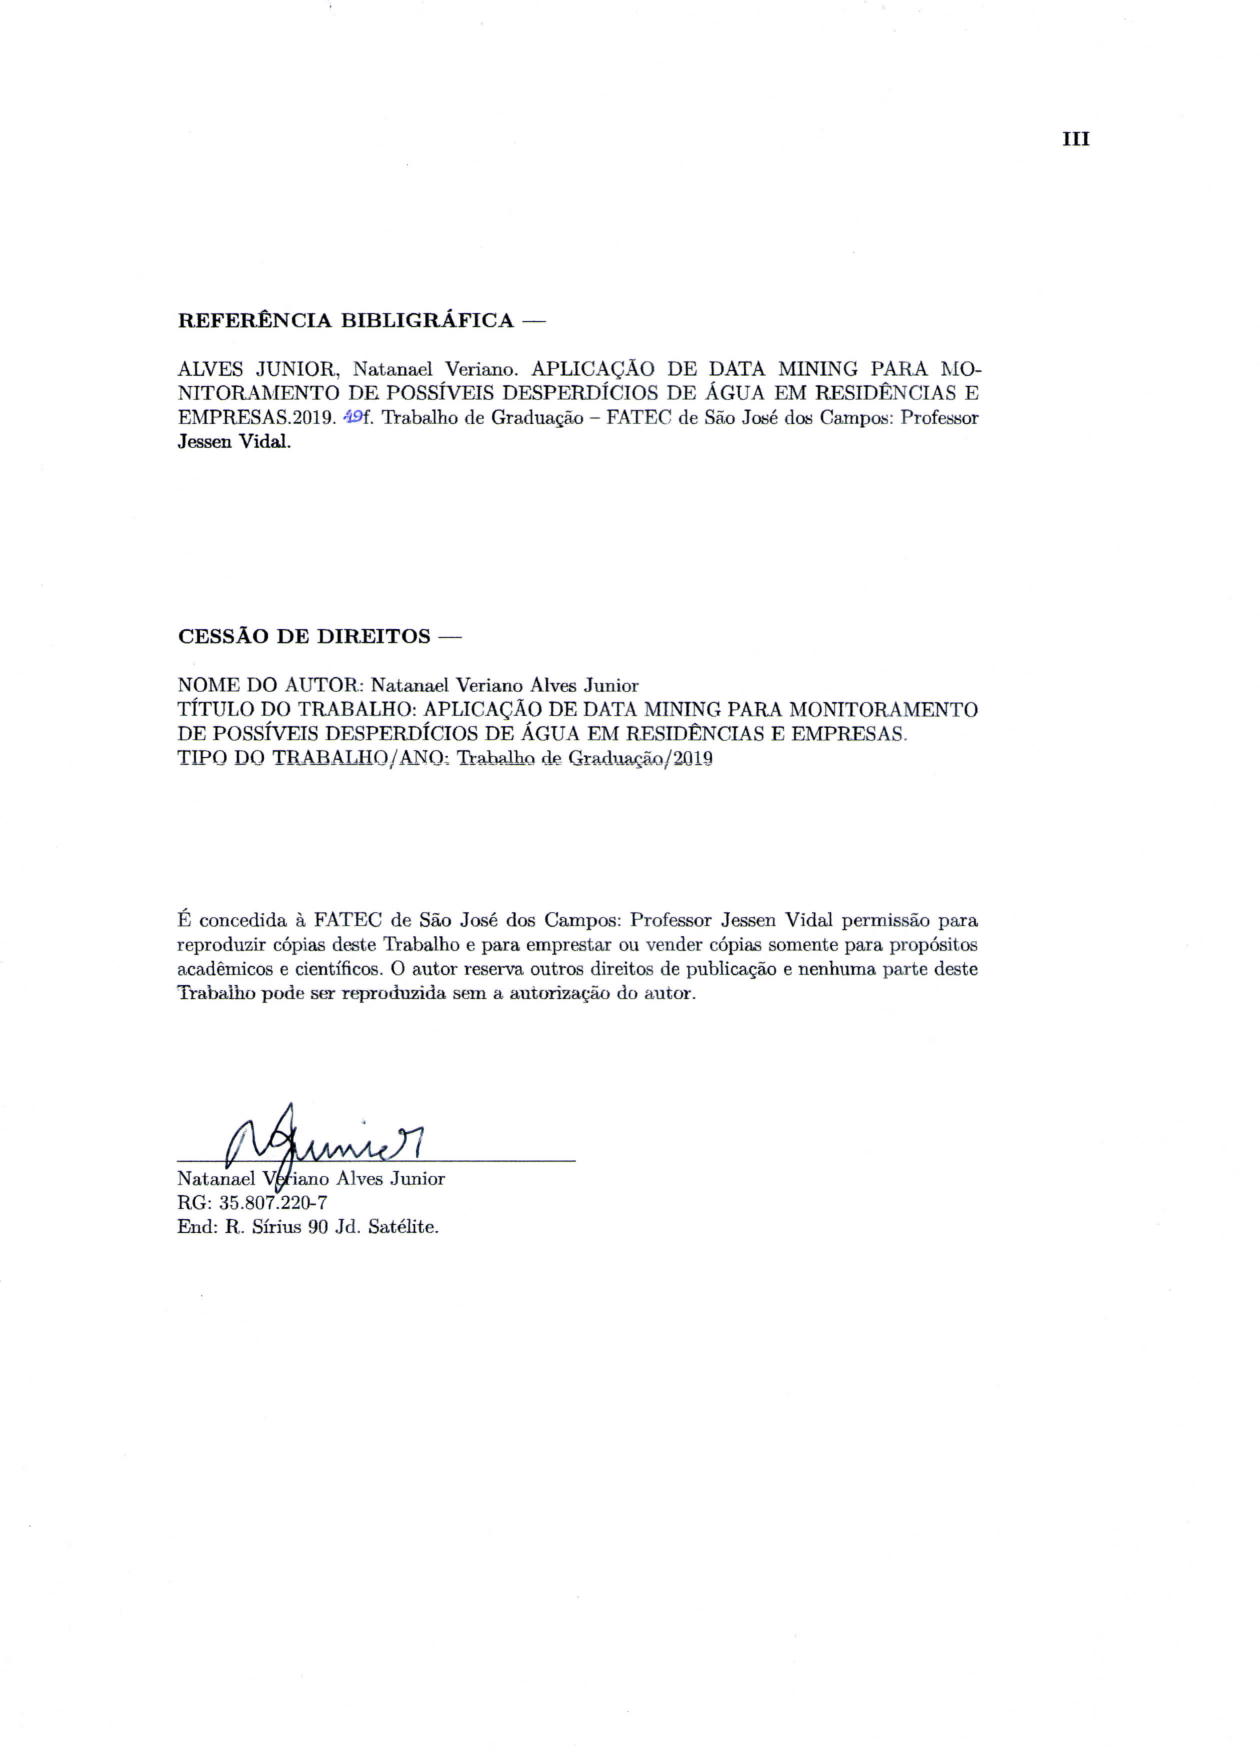
\includepdf{cessao_de_direitos2}%duas folhas
\end{fichacatalografica}

% ---
% Folha de aprovação
% ---
%edita folha de aprovacao
\begin{folhadeaprovacao}

  \begin{center}
    {\ABNTEXchapterfont\large\imprimirautor}

    \vspace*{\fill}\vspace*{\fill}
    \begin{center}
      \ABNTEXchapterfont\bfseries\Large\imprimirtitulo
    \end{center}
    \vspace*{\fill}

    \hspace{.45\textwidth}
    \begin{minipage}{.5\textwidth}
        \imprimirpreambulo
    \end{minipage}%
    \vspace*{\fill}
   
   \end{center}
%	\noindent\rule{7cm}{0.4pt}\\
\begin{center}


   \vspace*{0.5cm}
    \textbf{Composição da Banca}
\end{center}
  %\begin{center}
  
  \assinatura{\textbf{Gerson Da Penha Neto, Mestre – FATEC – SJC.} \\ Orientador\\}
   \vspace*{0.5cm}
   %{\textbf{\imprimircoorientador} \\ Coorientador\\\vspace*{0.5cm}}
%   \noindent\rule{15cm}{0.4pt}\\
  \assinatura{\textbf{Diogo Branquinho Ramos, Mestre, TECSUS – FATEC – SJC.} \\ Membro da Banca\\\vspace*{0.5cm}}
 %  \noindent\rule{15cm}{0.4pt}\\
\assinatura{\textbf{Emanuel Mineda Carneiro, Mestre, FATEC – SJC.} \\ Membro da Banca\\\vspace*{0.5cm}}
   %\assinatura{\textbf{Professor} \\ Convidado 4}
%\end{center} 
\vspace*{0.5cm}  
   \begin{center}
    \vspace*{0.5cm}
    {\large\imprimirlocal}
    \par
    {\large\imprimirdata}
    \vspace*{1cm}
  \end{center}

\end{folhadeaprovacao}
%inclui folha de aprovacao pdf
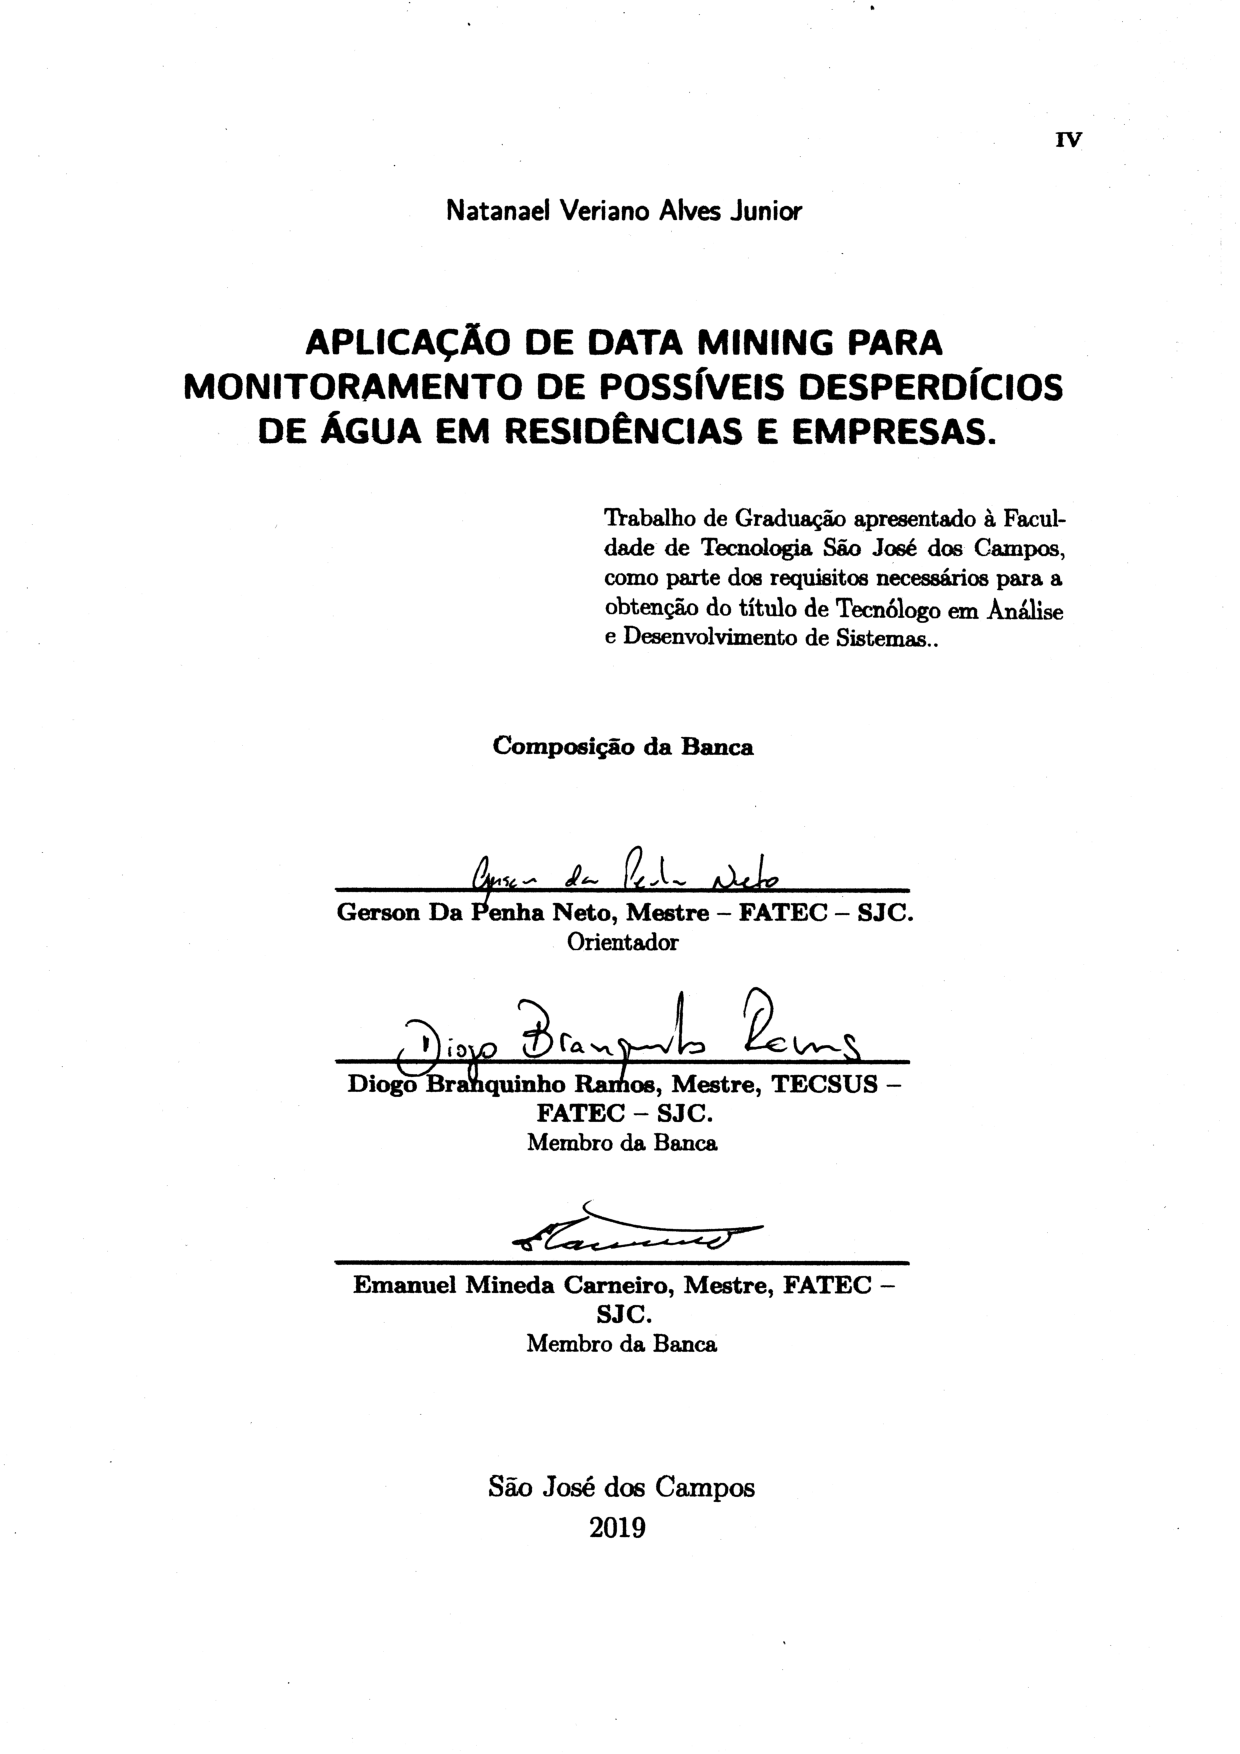
\includepdf[]{folhaAprov2.pdf}
% ---

% ---
% Dedicatória
% ---
\begin{dedicatoria}
   \vspace*{\fill}
   \begin{flushright}
   
   \textit{Dedico este trabalho primeiramente à Deus,
   \\ socorro presente na hora da angústia,
    \\minha esposa, aos meus pais e a minha filha.}
   %\textit{Nós não conseguimos o que merecemos,\\ só conseguimos o que é possível.} 
  
   \end{flushright}
\end{dedicatoria}



% ---

% ---
% Agradecimentos
% ---
\begin{agradecimentos}
\par Primeiramente agrade\c{c}o a Deus que permitiu que tudo isso acontecesse.
Também agrade\c{c} ao Professor Me. Eng. Gerson Da Penha Neto, pela orienta\c{c}\~ao , apoio e  confian\c{c}a.Ao Professor Me. Diogo Branquinho Ramos que proporcionou os dados para o estudo e tamb\'em o est\'agio supervisionado.\'A Institui\c{c}\~ao Faculdade de Tecnologia de S\~ao Jos\'e dos Campos (FATEC-SJC) pelo ambiente  amig\'avel  e criativo  que proporciona, e a quantidade imensur\'avel de conhecimento. \'A minha esposa Bruna e minha filha Lanna pelo amor, pela compreens\~ao, pelo aux\'ilio, pelo companheirismo.  Aos meus pais pelo amor, incentivo  e  apoio incondicional.
\par Minha eterna gratid\~ao  a  todos aqueles que colaboraram diretamente ou indiretamente para est\'a conquista que pode ser concretizada,  e  tamb\'em  agradeço a cria\c{c}\~ao do modelo de Trabalho de Gradua\c{c}\~ao para a FATEC-SJC utilizando \LaTeX.

\end{agradecimentos}
% ---

% ---
% Epigrafe
% ---
\begin{epigrafe}
    \vspace*{\fill}
    \begin{flushright}
%        \textit{''Eu acredito que os HotDogs simbolizam uma filosofia muito profunda, \\
%                na qual todos nós poderíamos ter a oportunidade de observá-la e aprendê-la. \\
%                O pão pode significar tudo que dá a nossa base para a nossa vida. \\
%                E a salsicha pode simbolizar nós mesmos, ou um simples conceito ou coisa que surge de uma epifania.''\\
%                (Rodrigo Takeshi, 26 de Outubro de 2016)}

        \textit{\\“Até aqui nos ajudou o Senhor.” 
\\1 Samuel 7:12.”\\
 }
    \end{flushright}
\end{epigrafe}
% ---

% ---
% RESUMOS
% ---
% resumo em português
\setlength{\absparsep}{18pt} % ajusta o espaçamento dos parágrafos do resumo
% --- resumo em português ---
\begin{resumo}
O Estado de São Paulo sofreu em 2014 com problemas da crise hídrica e assim despertou-se a necessidade de armazenamento e o consumo inteligente de água.
A empresa TecSUS, visando à sustentabilidade, desenvolve tecnologias que ajudam na economia dos recursos. Entre seus produtos se destaca TecHydro, equipamento que faz a captação dos dados de consumo de água. A empresa TecSUS com os dados obtidos, necessitava de uma análise para uma possível detecção de vazamento e  excesso no consumo de água, visando economia de água. Assim inicia-se um estudo com os dados utilizando algumas técnicas de \emph{Data Mining}, ou melhor, Mineração de Dados, com ferramentas e bibliotecas \emph{open source}, com a linguagem de programação \emph{Python} e com utilização do \emph{Jupyter Notebook} que é uma ferramenta \emph{Web} que auxilia na integração dos algoritmos, das bibliotecas e facilita a visualização dos resultados.
E com aplicação da fórmula matemática da Distância Euclidiana, verificou que houve períodos sem consumo de água e sendo assim podendo constatar de que nesses períodos não houve vazamento de água.
    
    \vspace{\onelineskip}
    \noindent
    \textbf{Palavras-chave}: Data Mining; Distância Euclidiana; TecHydro; \emph{Jupyter Notebook}; \emph{Python}.
\end{resumo}

% resumo em inglês
\begin{resumo}[Abstract]
    \begin{otherlanguage*}{english}

\textit{
The State of São Paulo suffered in 2014 with problems of the water crisis and thus the need for storage and the intelligent consumption of water was awakened.
 The TecSUS company, aiming at sustainability, develops technologies that help in saving resources. Among its products stands out TecHydro, equipment that captures water consumption data. The company TecSUS with the obtained data, needed an analysis for a possible detection of leakage and excess in the consumption of water, aiming at saving water. Thus, a study of the data using some techniques of Data Mining, or better, Data Mining, with tools and open source libraries, with the programming language Python and with using the Jupyter Notebook which is a Web tool that helps in the integration of algorithms, libraries and facilitates the visualization of the results.
 And with the application of the mathematical formula of Euclidean Distance, it was verified that there were periods without water consumption and being thus able to verify that in those periods there was no water leakage.
}%

	    \vspace{\onelineskip}
	    \noindent
	    \\
	    \textbf{Keywords}: Data Mining; Distância Euclidiana; TecHydro; Jupyter Notebook; Python.
    \end{otherlanguage*}
\end{resumo}
% ---

% ---
% inserir lista de ilustrações
% ---
\pdfbookmark[0]{\listfigurename}{lof}
\listoffigures*
\cleardoublepage
% ---

% ---
% inserir lista de tabelas
% ---
\pdfbookmark[0]{\listtablename}{lot}
\listoftables*
\cleardoublepage
% ---

% ---
% inserir lista de abreviaturas e siglas
% ---
\begin{siglas}
	\item[SABESP]   			\emph{Companhia de Saneamento Básico do Estado de São Paulo}
	\item[ANA]  	    		\emph{Agência Nacional de Águas}
	\item[MQTT] 				\emph{Message Queuing Telemetry Transport}
	\item[UHE Funil] 			\emph{Usina Hidrelétrica Funil}
	\item[UHE Jaguari] 			\emph{Usina Hidrelétrica Jaguari}
	\item[UHE Paraibuna] 		\emph{Usina Hidrelétrica Paraibuna}
	\item[UHE Santa Branca] \emph{Usina Hidrelétrica Santa Branca}
	\item[BSD] 					\emph{Berkeley Software Distribution}
	\item[IDE]				    \emph{Integrated Development Environment}
	\item[KDD]					\emph{Knowledge Discovery in Databases}
	\item[GNU] 					\emph{General Public License}


\end{siglas}
% ---

% ---
% inserir lista de símbolos
% ---
\begin{simbolos}

  \item[D] Distância Euclidiana

\end{simbolos}
% ---
% ---
% inserir o sumario
% ---
\pdfbookmark[0]{\contentsname}{toc}
\tableofcontents*
\cleardoublepage
% ---

% ----------------------------------------------------------
% ELEMENTOS TEXTUAIS
% ----------------------------------------------------------

\textual

\setcounter{page}{15}
% ---
% Incluindo Capitulo 1 - Introducao
% ---
% ----------------------------------------------------------
% Introdução (exemplo de capítulo sem numeração, mas presente no Sumário)
% ----------------------------------------------------------
\chapter[Introdução]{Introdução}
%\addcontentsline{toc}{chapter}{Introdução}
% ----------------------------------------------------------
\par O Estado de São Paulo sofreu com problemas da crise hídrica, decorrente pelo fato do consumo excessivo e uso inconsciente da água  dentre outros fatores. Esse problema afetou também a região do Vale do Paraíba, como pode ser observado no relatório da ANA \cite{ana1}, onde o Sistema Hidráulico Paraíba do Sul observou uma redução acelerada dos níveis das represas e esteve operando meses em estado de alerta. Assim foi tomada atitude mais emergenciais como intensificar as manobras de redução de pressão e também o bombeamento do volume morto, com águas mais sujas que ficam no fundo das represas, e também pedir para população se conscientizar e racionar o consumo de água.

 
\begin{figure}[h]
	\caption{\textbf{Volume Útil dos Reservatórios do Sistema Hidráulico Paraíba do Sul}}
	\centering
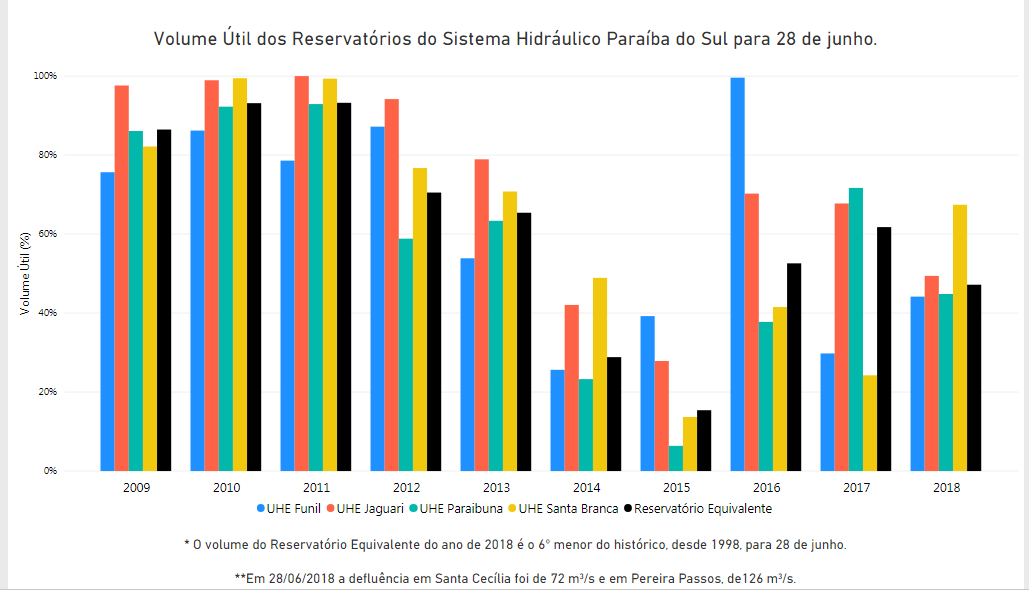
\includegraphics[width=\textwidth,height=\textheight ,keepaspectratio]{figuras/situacaoreservatoriosvaleparaiba}
    \label{fig:ana}	
	\fonte{Adaptada pelo autor, de \citeonline{ana1}}
\end{figure}



% ######## init table ########
\begin{table}[ht]
\caption{ \textbf{Dados dos Volumes Útil dos Reservatórios do Sistema Hidráulico Paraíba do Sul}}
\centering
\begin{tabular}{|c|c|c|c|c|c|}
\hline
\rowcolor[HTML]{80C397} 
\textbf{ANO}                          & \textbf{\begin{tabular}[c]{@{}c@{}}UHE \\ Funil\end{tabular}} & \textbf{\begin{tabular}[c]{@{}c@{}}UHE\\  Jaguari\end{tabular}} & \textbf{\begin{tabular}[c]{@{}c@{}}UHE\\  Paraibuna\end{tabular}} & \textbf{\begin{tabular}[c]{@{}c@{}}UHE\\  Santa Branca\end{tabular}} & \textbf{\begin{tabular}[c]{@{}c@{}}Reservatório \\ Equivalente\end{tabular}} \\ \hline
\textbf{2009}                         & \textbf{75,66\%}                                              & \textbf{97,62\%}                                                & \textbf{86,10\%}                                                  & \textbf{82,18\%}                                                     & \textbf{86,47\%}                                                             \\ \hline
\rowcolor[HTML]{80C397} 
\textbf{2010}                         & \textbf{86,21\%}                                              & \textbf{98,95\%}                                                & \textbf{92,26\%}                                                  & \textbf{99,45\%}                                                     & \textbf{93,15\%}                                                             \\ \hline
\textbf{2011}                         & \textbf{78,60\%}                                              & \textbf{103,11\%}                                               & \textbf{92,92\%}                                                  & \textbf{99,36\%}                                                     & \textbf{93,24\%}                                                             \\ \hline
\rowcolor[HTML]{80C397} 
\textbf{2012}                         & \textbf{87,20\%}                                              & \textbf{94,18\%}                                                & \textbf{58,84\%}                                                  & \textbf{76,72\%}                                                     & \textbf{70,51\%}                                                             \\ \hline
\textbf{2013}                         & \textbf{53,87\%}                                              & \textbf{78,93\%}                                                & \textbf{63,36\%}                                                  & \textbf{70,78\%}                                                     & \textbf{65,40\%}                                                             \\ \hline
\rowcolor[HTML]{80C397} 
\textbf{2014}                         & \textbf{25,63\%}                                              & \textbf{42,06\%}                                                & \textbf{23,27\%}                                                  & \textbf{48,92\%}                                                     & \textbf{28,84\%}                                                             \\ \hline
\cellcolor[HTML]{FFFFFF}\textbf{2015} & \textbf{39,23\%}                                              & \textbf{27,87\%}                                                & \textbf{63,80\%}                                                  & \textbf{13,69\%}                                                     & \textbf{15,40\%}                                                             \\ \hline
\rowcolor[HTML]{80C397} 
\textbf{2016}                         & \textbf{99,60\%}                                              & \textbf{70,25\%}                                                & \textbf{37,77\%}                                                  & \textbf{41,53\%}                                                     & \textbf{52,59\%}                                                             \\ \hline
\textbf{2017}                         & \textbf{29,78\%}                                              & \textbf{67,75\%}                                                & \textbf{71,69\%}                                                  & \textbf{24,24\%}                                                     & \textbf{61,77\%}                                                             \\ \hline
\rowcolor[HTML]{80C397} 
\textbf{2018}                         & \textbf{44,16\%}                                              & \textbf{49,42\%}                                                & \textbf{44,84\%}                                                  & \textbf{67,43\%}                                                     & \textbf{47,18\%}                                                             

\end{tabular}
\label{table:table_ana}
\fonte{Adaptada pelo autor, de \citeonline{ana1}}
\end{table}
  	
 
\par O problema pode ser observado na figura \ref{fig:ana} e na tabela \ref{table:table_ana}, visualizando os níveis dos reservatórios que oscilam, isso é alarmante. Visto isso, a empresa TecSUS Tecnologias para a Sustentabilidade desenvolveu tecnologias que ajudam na economia dos recursos escassos do planeta e aumentam a eficiência de processos e produtos. Com produto TecHydro, monitoramento e controle remoto de hidrômetros, podendo ser para uso doméstico, comercial e industrial. A coleta de dados de consumo de água em intervalos pré-programados (entre 1 minuto e 24 horas). Com os dados obtidos, a empresa analisa o consumo e gera um relatório.

\par 


\section{Motivação}
\par Foi escolhido esse tema para realizar um estudo no consumo de água para investigação de detecção possível excesso e vazamento em residências e empresas, com aplicação de \emph{data mining}, visando economia no consumo de água.
\section{Objetivos}
\par As subseções a seguir apresentam os objetivos deste trabalho.
\subsection{ Objetivo Geral}
\par Este trabalho de graduação tem por objetivo desenvolver um estudo para se identificar possíveis desperdícios de água em residências e empresas, com aplicação de \emph{data mining}, visando economia no consumo de água.
\subsection{Objetivo Específico}
\par Para a realização deste  foram estabelecidos os objetivos específicos:
\begin{itemize}
	\item Realizar a captação de dados no estilo xlsx;
	\item Fazer a mineração dos dados coletados;
	\item Fazer a análise dos dados coletados;
	\item Fazer a plotagem dos dados coletados em gráficos;
\end{itemize}


% ---

% ---
% Incluindo Capitulo 2 - Fundamentacao Teorica
\chapter{Contextualização Tecnológica}



\section{A Empresa TecSus}
\par A Empresa TecSUS Tecnologias para a Sustentabilidade, é uma \emph{startup} de tecnologia da informação que atua no desenvolvimento de dispositivos, aplicativos e sistemas para transmissão e recepção de dados, controle de equipamentos remotos e gestão da informação, aplicados predominantemente nos setores de abastecimento de água, saneamento, geração e distribuição de eletricidade, distribuição de gás natural, e serviços municipais, embora as aplicações possam ter caráter mais abrangente. As tecnologias visam aprimorar o uso dos recursos naturais do planeta, contribuindo para a redução do desperdício (de água, energia, gás e tempo) e tornando a gestão destes recursos mais eficiente.


\section{A Coleta dos dados}
\par A Empresa TecSUS coleta informações para monitoramento de consumo de água. O serviço é oferecido tanto para residências como para estabelecimentos comerciais. Veja a ilustração do serviço prestado na figura \ref{techid}.
\begin{figure}[ht]
	\caption{\textbf{TecHydro Monitoramento e Controle remoto de hidrômetros}}
	\centering
		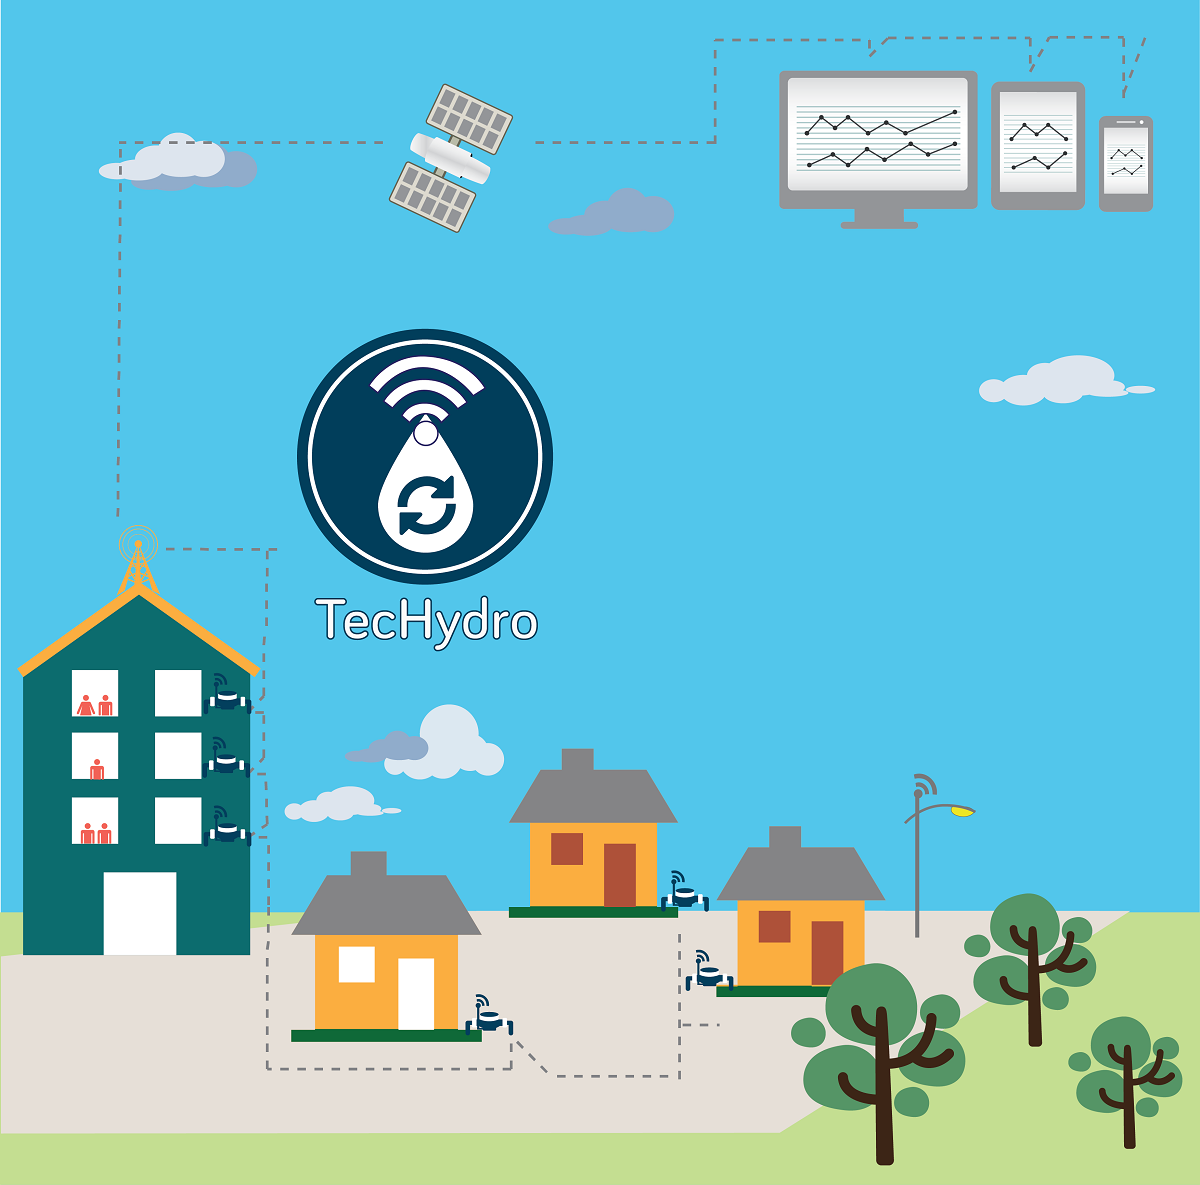
\includegraphics[scale=0.3]{figuras/TecHydro}
	\fonte{TecSUS(2018).}
	\label{techid}
\end{figure}

\par Os dados são coletados diretamente dos hidrômetros, por uma placa eletrônica da TecSus. Esses dados são transmitidos em uma rede \emph{mesh} local, até chegar a um concentrador de dados que fica no cliente.
\par O concentrador de dados tem acesso à \emph{internet} e enviam esses dados para a nuvem através de MQTT \emph{(Message Queuing Telemetry Transport)}, os dados quando chegam à nuvem são processados e armazenados no banco de dados.


\section{Dados e Informação}

\par Com é explicado em  \cite{Elias}, os dados não tem  significado relevante não conduz uma compreensão com exatidão, os dados podem ser com exemplo uma \emph{string} ou um caractere numérico ou alfabético ou simbolos e caracters especiais.
\par E a informação é a ordenação e a organização dos dados de forma que transmita um significado ou uma compreensão dentro de um determinado contexto. O conjunto ou consolidação dos dados de forma a fundamentar o conhecimento.
\par Quanto mais distanciamos dos dados maior é a abstração, como pode ser observado na figura \ref{abst}
\begin{figure}[ht]
	\caption{\textbf{Abstração}}
	\centering
		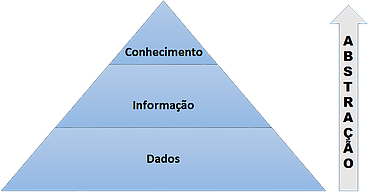
\includegraphics[width=\textwidth,height=\textheight, keepaspectratio]{figuras/abstracao}
		\label{abst}
	\fonte{\cite{Elias}}
\end{figure}


\section{\emph{Data Mining} (Mineração de Dados) e KDD}
%\label{minerdados}

\subsection{\emph{Data Mining} (Mineração de Dados)}

\par A mineração de dados geralmente faz parte de uma maior inteligência de negócios ou gerenciamento de conhecimento
iniciativa conforme é explicado em \cite{dig2004privacy}. Como os governos estaduais são organizações complexas que coletam e processam grandes quantidades de informações, a mineração de dados pode ajudar a fornecer valor ao governo estadual operações e contribuintes através da extração de informações úteis das montanhas de
dados. Além disso, a mineração de dados pode ser preditiva e descobrir padrões ocultos que
pode estrategicamente usar para reduzir custos, aumentar as oportunidades de expansão de negócios, e detectar fraudes, desperdícios e abusos que drenam os dólares dos contribuintes.
\par O objetivo da mineração de dados é identificar padrões para fazer previsões a partir de
informações contidas em bancos de dados. Ele permite que o usuário seja proativo na identificação e predizendo tendências com essa informação. Usos comuns de mineração de dados no governo incluem descoberta de conhecimento, detecção de fraudes, análise de pesquisa, suporte à decisão e personalização do site. Os usos mais comuns do governo federal de mineração de dados
identificados pelo GAO(U.S. General Accounting Office (GAO)) incluem:
\begin{itemize}
\item Melhorar o serviço ou desempenho
\item Detectar fraude, desperdício e abuso
\item Analisar informações científicas e de pesquisa
\item Gestão de recursos humanos
\item Detectar atividades ou padrões criminosos
\item Analisar inteligência e detectar atividades terroristas
\end{itemize}

\subsection{KDD \emph{(Knowledge Discovery in Databases)}}

\par O processo capaz de descobrir conhecimento (informação) em banco de dados chama-se KDD \emph{(Knowledge Discovery in Databases)}, este processo foi proposto em 1989 por\cite{fayyad1996data}, para referir-se as etapas que produzem conhecimento a partir de dados. Dentro deste processo a etapa de mineração de dados é a fase que transforma dados em informação.
\par Definida como o processo de descoberta de padrões nos dados por  \cite{fayyad1996data}, com o objetivo de explicar a informação e a realizar predições a partir da mesma. A prática de mineração de dados tem como objetivo produzir informação na forma de fatos ou padrões, também chamados conhecimento adquirido segundo \cite{fayyad1996data}. Este conhecimento para ser corretamente interpretado e útil, deve ser apresentado de forma a atingir tal propósito, apresentando assim o que foi aprendido para poder realizar reflexões a partir do mesmo. Pode se observar os processos do KDD com mais clareza na figura \ref{kdd} .
\begin{figure}[h]
	\caption{\textbf{Etapas do processo KDD}}
	\centering
		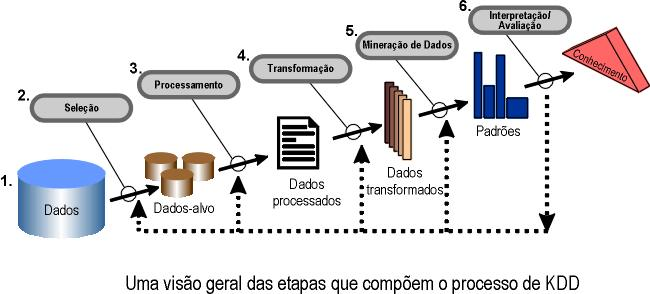
\includegraphics[width=\textwidth,height=\textheight, keepaspectratio]{figuras/processo de kdd.jpg}
		\label{kdd}
	\fonte{\cite{fayyad1996data}}
\end{figure}
\par O processo inicia-se com a obtenção dos dados. Depois etapa de seleção, é onde serão decididos quais os conjuntos de dados que serão relevantes para que sejam obtidos resultados com informações uteis. Na etapa de processamento acontece à limpeza dos dados e seleção de atributos. Nesta etapa informações ausentes errôneas ou inconsistentes nas bases de dados devem ser corrigidas de forma a não comprometer a qualidade dos modelos de conhecimento a serem extraídos ao final do processo de KDD. A etapa de transformação dos dados analisa os dados obtidos da etapa anterior e os reorganiza de uma forma especifica para que possam ser interpretados na etapa seguinte. Na etapa de mineração dos dados é onde tudo acontece, os dados depois de transformados serão lidos e interpretados. A mineração faz com que meros dados sejam transformados em informações, tais informações são indicadas através de força bruta, ou seja, lendo regra por regra e as interpretando. Na última etapa a de interpretação de resultados é onde as regras indicadas pelo processo anterior serão interpretadas e avaliadas. 
\section{Distância Euclidiana}
%\label{distan}
\par A distância euclidiana é uma medida de Dissimilaridade, é um conceito matemático que representa a menor distância existente entre dois pontos na Geometria Euclidiana. Esta geometria foi construída pelo matemático grego Euclides. Segundo  \cite{regazzi2002analise}, “embora a distância euclidiana seja uma medida de dissimilaridade, às vezes ela é referida como uma medida de semelhança, pois quanto maior seu valor, menos parecidos são os indivíduos ou unidades amostrais”, quanto menor o valor observado mais parecido serão os objetos ou nesse caso os pontos da série temporal. A Distância Euclidiana só pode ser medida em séries do mesmo tamanho, consistindo no cálculo da distância entre os pares de pontos das duas sequencias.
\par O calculo  tem complexidade O(n), mas pode ser acelerado. Quando ela é utilizada como sub-rotina em algoritmos de mineração como o de classificação, por exemplo, o interesse pode estar em conhecer a verdadeira distância entre séries.
\par De acordo com \cite{manly2016multivariate}, “a distância euclidiana, quando for estimada a partir das variáveis originais, apresenta a inconveniência de ser influenciada pela escala, de medida pelo número de variáveis e pela correlação existente entre as mesmas”. Para contornar as escalas, faz-se a padronização das variáveis em estudo, para que possuam a variância igual à unidade.
\par Distância entre duas instâncias $P_i$ e $P_j$ definida como:
\begin{figure}[ht]
\caption{\textbf{Distância Euclidiana}}
\centering

    \newlength\dlf
    \newcommand\alignedbox[2]{
      % #1 = before alignment
      % #2 = after alignment
      &
      \begingroup
      \settowidth\dlf{$\displaystyle #1$}
      \addtolength\dlf{\fboxsep+\fboxrule}
      \hspace{-\dlf}
      \fcolorbox{black}{gray!30}{$\displaystyle #1 #2$}
      \endgroup
    }

    \begin{align}\
        \alignedbox{}{D=\sqrt{ \sum\limits_{k=1}^n (P_{ik}-P_{jk})^2}}
    \end{align}
       \label{distancia_euclidiana}
       \fonte{\cite{manly2016multivariate}}
    \end{figure}

\par $P_{ik}$ e $P_{jk}$ para K = 1..., n. São os n que descrevem as instâncias $p_i$ e $p_j$, respectivamente.
\par A distância euclidiana é, sem dúvida, a medida de distância mais utilizada para a análise de agrupamentos e para análise de séries temporal. Considerando o caso mais simples, no qual existem n indivíduos, onde cada um dos quais possuem valores para p variáveis, a distância euclidiana entre eles é obtida mediante o teorema de Pitágoras, para um espaço multidimensional.
\par Explicando a formula, é a raiz quadrada da soma dos resultados da diferença entre os pontos elevados ao quadrado, pode ser observada na figura \ref{distancia_euclidiana}. 

\section{Linguagem Python, e suas bibliotecas e ferramentas}

\par Para ter mais eficiência na análise de dados foi utilizada a linguagem \emph{Python} e também utiliza-se algumas bibliotecas destinadas para análise de dados e cálculos específicos.
\par O \emph{ \cite{python}} é uma linguagem de programação criada por \emph{Guido Van Rossum} em 1991,  é a linguagem ideal para aplicações científica sendo uma linguagem expressiva, em que é fácil traduzir o raciocínio em um algoritmo e tem sido ótimo para dados e preparação, e para análise e modelagem de dados.
\par A \cite{pandas}  é uma biblioteca \emph{open source}, licenciada pelo BSD, que por sua vez é uma licença de código aberto inicialmente utilizada nos sistemas operacionais do tipo \emph{Berkeley Software Distribution}, que fornece estruturas de dados de alto desempenho e fáceis de usar e ferramentas de análise de dados para a linguagem de programação \emph{Python}. A biblioteca ajuda a preencher essa lacuna, permitindo que você execute todo o seu fluxo de trabalho de análise de dados em Python sem precisar alternar para um idioma mais específico do domínio, como Linguagem R. Combinado com o excelente \emph{kit} de ferramentas \emph{IPython} e outras bibliotecas, o ambiente para análise de dados no Python se destaca no desempenho, produtividade e capacidade de colaboração. 
\par A biblioteca \cite{numpy} é descrita  como o pacote básico da linguagem \emph{Python} que permite trabalhar com arranjos, vetores e matrizes de N dimensões, de uma forma comparável e com uma sintaxe semelhante ao \emph{software} proprietário \emph{Matlab}, mas com muito mais eficiência, e com toda a expressividade da linguagem.
\par A biblioteca \emph{ \cite{matplotlib}}, é uma biblioteca de plotagem 2D em \emph{Python} que produz números de qualidade de publicação em uma variedade de formatos impressos e ambientes interativos entre plataformas. O \emph{Matplotlib} pode ser usado em \emph{scripts Python}, nos \emph{shells} do \emph{Python} e do \emph{IPython}, no \emph{Notebook Jupyter}, nos servidores de aplicativos da \emph{Web} e em quatro \emph{kits} de ferramentas de interface gráfica do usuário.
\par  E   para fazer a integração da linguagem \emph{python} com as bibliotecas, pode-se utilizar vários compiladores, IDE (\emph{Integrated Development Environment})  que   \'e o  Ambiente de Desenvolvimento Integrado,  \emph{Pycharm}, \emph{Visual Studio}, \emph{Notepad++} e o \emph{Jupyter Notebook}, onde o mesmo foi utilizado para a análise dos dados e plotagem dos gráficos. 
\par O \emph{ \cite{jupyter}}, a explicação que é um aplicativo da \emph{Web} de código aberto que permite criar e compartilhar documentos que contêm código ativo, equações, visualizações e texto narrativo. Os usos incluem: limpeza e transformação de dados, simulação numérica, modelagem estatística, visualização de dados, aprendizado de máquina e muito mais. Nascido do Projeto \emph{IPython} em 2014, à medida que evoluiu para suportar ciência de dados interativa e computação científica em todas as linguagens de programação.   
% ---

% ---
% Incluindo Capitulo 3 - Desenvolvimento
	\newpage
\chapter{DESENVOLVIMENTO DO TRABALHO}

\par Objetivo desse capítulo é apresentar o desenvolvimento e a implantação do algoritmo para análise de dados.



\section{Coleta dos Dados}

\par Os dados depois de coletados e armazenados foram concedidos uma pequena amostra, mais ou menos oito meses de dados, no formato de xlsx (planilha \emph{Excel}) como pode ser observada na figura \ref{arquivo_de_dados}. Os dados têm  as informações de data hora da coleta a quantidade de litros consumidos por hora, e o total de litros acumulados. Com os dados em mãos foi inserido no \emph{jupyter notebook}, para realizar alguns experimentos, de \emph{data mining} com linguagem \emph{python} e suas bibliotecas.

\begin{figure}[ht]
	\caption{\textbf{Arquivo de Dados formato \emph{Excel}}}
	\centering
		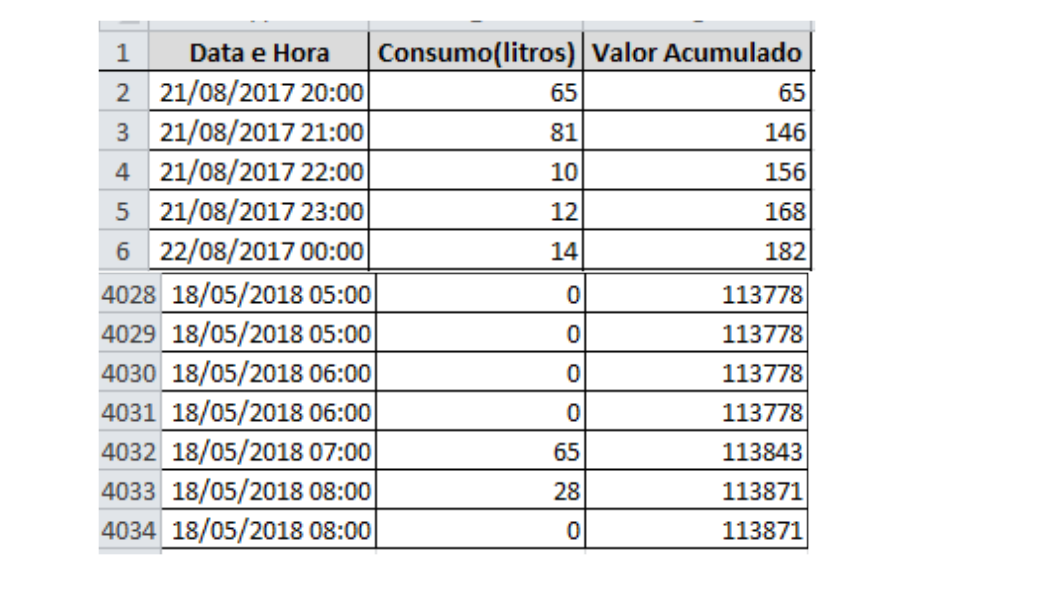
\includegraphics[width=\textwidth,height=\textheight, keepaspectratio]{figuras/planilhaexceldosdados3.png}
		\label{arquivo_de_dados}
	%\fonte{\cite{fayyad1996data}}
\end{figure}


\section{Desenvolvimento do algoritmo}

\begin{figure}[ht]
	\caption{\textbf{Importando as Bibliotecas}}
	\centering
		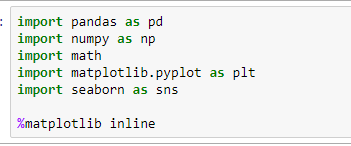
\includegraphics[scale=1, keepaspectratio]{figuras/importacaodasbibliotecas.PNG}
		\label{impor_b}
	%\fonte{\cite{fayyad1996data}}
\end{figure}

\par Como pode ser visualizado na figura \ref{impor_b}, o primeiro passo que deve ser feito é a importação das devidas bibliotecas para a análise dos dados. E é acrescentado um algoritmo na última linha o \emph{"\%matplotlib inline"} este por sua vez serve auxiliar a visualização na apresentação dos gráficos no \emph{jupyter notebook} sem a necessidade de utilizar a função especifica sendo está a \emph{“plt.show()”}.


\begin{figure}[ht]
	\caption{\textbf{Importação do arquivo}}
	\centering
		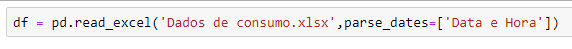
\includegraphics[scale=1, keepaspectratio]{figuras/importaroarquivo}
		\label{impor_arquivo}
	%\fonte{\cite{fayyad1996data}}
\end{figure}


\par Na figura \ref{impor_arquivo},  é   feita  a  importação do arquivo com os dados, atribui-se o arquivo com os dados a uma variável. Neste caso a variável denominada de "df", o  nome é dado comumente a uma variável, pois é a iniciais de um \emph{data frame}. Por sua vez um data frame é semelhante a uma matriz, mas as suas colunas tem nomes e podem conter dados de tipos diferentes. Um \emph{data frame} pode ser visto como uma tabela de uma base de dados, em que cada linha corresponde a uma registro da tabela. Cada coluna corresponde às propriedades, ou campos, a serem armazenadas para cada registro da tabela.  E   após  o  nome do arquivo  e  tipos do arquivo foi colocado uma função, \emph{"$parse_dates$"}, onde verifica a se as datas estão em um formato adequado para criação do \emph{data frame}.

\begin{figure}[ht]
	\caption{\textbf{Mostrando conteúdo do Data Frame}}
	\centering
		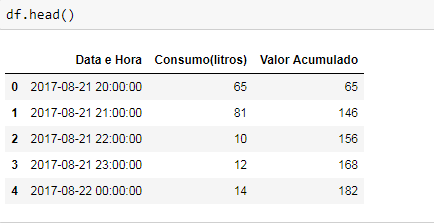
\includegraphics[scale=1, keepaspectratio]{figuras/mostraroconteudodoarquivo}
		\label{conteudo_df}
	%\fonte{\cite{fayyad1996data}}
\end{figure}

\par Ao executar este comando \emph{"df.head()"} podendo observar na figura \ref{conteudo_df}, é o conteúdo do \emph{data frame}. Verificando que o arquivo contém linhas e colunas, e que nas colunas compreende que contém data e hora em que o dado foi extraído, outra coluna a quantidade de litros de água consumidos e na outra coluna o valor acumulado de litros, a partir dá primeira extração dos dados. 

\begin{figure}[ht]
	\caption{\textbf{Separação da coluna Data e Hora}}
	\centering
		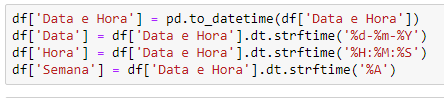
\includegraphics[scale=1, keepaspectratio]{figuras/organizararquivopordata}
		\label{separar_horaedata}
	%\fonte{\cite{fayyad1996data}}
\end{figure}

\par Após verificar o conteúdo do \emph{data frame}, é aplicado um algoritmo para desmembrar a coluna Data e Hora e criar outras colunas, como pode se observar na figura \ref{separar_horaedata}. Onde cada coluna recebeu os dados de acordo com as suas descrições, a coluna Data recebeu somente as datas, a coluna Hora recebeu somente as horas e foi criada uma coluna denominada de Semana, onde recebeu os dias da semana referenciando com a coluna Data.
\begin{figure}[ht]
	\caption{\textbf{Data Frame modificado}}
	\centering
		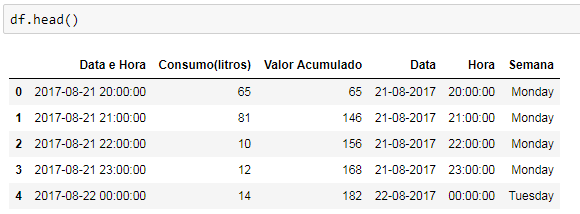
\includegraphics[scale=1, keepaspectratio]{figuras/mostrandoarquivoaposorganizacao}
		\label{arquivo_orga}
	%\fonte{\cite{fayyad1996data}}
\end{figure}

\par Na figura \ref{arquivo_orga} trata-se do \emph{data frame} que foi modificado para que as análises fossem realizadas com mais exatidão possível.

\begin{figure}[ht]
	\caption{\textbf{Funções \emph{Describe e mean}}}
	\centering
		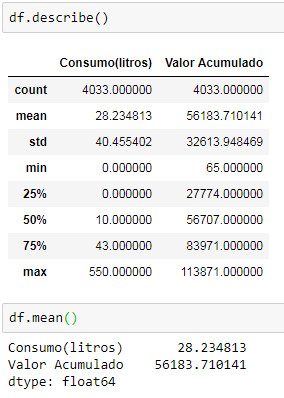
\includegraphics[scale=1, keepaspectratio]{figuras/describe-mean}
		\label{describe_mean}
	%\fonte{\cite{fayyad1996data}}
\end{figure}

\par Aplicando-se a função \emph{“df.describe”} no \emph{data frame}, como pode notar na figura \ref{describe_mean}, há o retorno de alguns dados estatísticos, onde o \emph{count} retorna a somatória de dados nesse caso total de 4033 dados para ambas as colunas, no caso do\emph{ mean} há o retorno das medias para todo o data frame, para a coluna consumo (litros) retorno de aproximadamente de 28 litros e na coluna valor acumulado o retorno de aproximadamente 56183 litros, onde se pode verificar o mesmo resultado a utilizar a função \emph{“df.mean()” } separadamente. No retorno do \emph{std}, que seria o desvio padrão, há o retorno na coluna de consumo (litros) de 40.455 e na coluna valor acumulado 32613.94. No caso do \emph{min} há o retorno de 0 litros na coluna de consumo (litros) e 65 na coluna valor acumulado, e no caso do \emph{“df.max ()”} há o retorno de 550 litros na coluna de consumo(litros) e 113871 na coluna de valor acumulado.

\begin{figure}[ht]
	\caption{\textbf{Algoritmo para plotagem dos dados}}
	\centering
		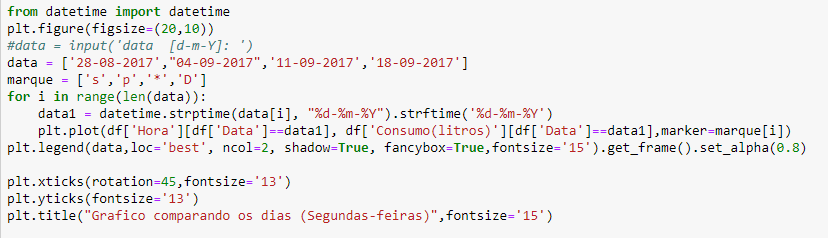
\includegraphics[width=\textwidth,height=\textheight , keepaspectratio]{figuras/codigograficoempython}
		\label{codigo_plotagem}
	%\fonte{\cite{fayyad1996data}}
\end{figure}

\par O Algoritmo na figura \ref{codigo_plotagem}, é utilizado para a plotagem dos dados, isso é o algoritmo serve para a visualização dos dados em forma de gráficos. Houve a importação da biblioteca \emph{datetime do python} para que se possa trabalhar com as datas. A função \emph{“plt.figure()”} é utilizada para formatar o tamanho da figura. Após é criada uma lista com algumas datas é atribuída a uma variável com nome de “data”, é feito o mesmo com a variável “marque”, mas recebendo uma lista com \emph{strings}, e com elas serão formados os marcadores do gráfico. Com um \emph{“for”} é feito uma iteração onde é passa por todos os elementos da lista “data”, e são adicionadas as datas separadas em uma variável “data1” onde é feita o tratamento para que possa ser realizada a plotagem de cada data na função \emph{“plt.plot()”}, se sendo assim também há iteração da lista dos marcadores onde cada data será plotada no gráfico tendo um marcador diferente, podendo assim fazer a comparação de cada data. E na função \emph{“plt.legend()”} é configurada a legenda do gráfico onde se podem ver os dados das datas diferente e realizando a comparação. Nas funções \emph{“plt.xticks”} e \emph{“plt.yticks()”} são configuradas os rótulos do gráfico tanto na horizontal como na vertical, ambas com o mesmo tamanho de fonte, mas o rotulo da horizontal tem uma pequena diferença a configuração da rotação dos rótulos para 45º para facilitar a visualização. E por fim \emph{“plt.title()”} onde é configurado o título do gráfico com a fonte tamanho 15. 

\begin{figure}[ht]
	\caption{\textbf{Função para calculo das médias diárias}}
	\centering
		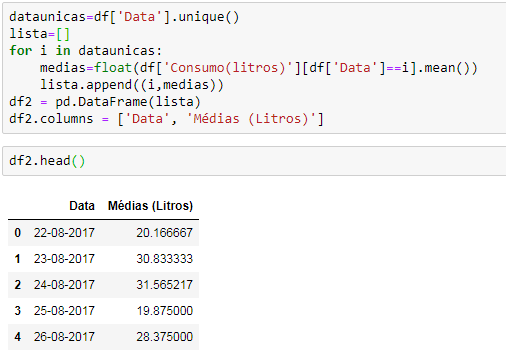
\includegraphics[scale=1, keepaspectratio]{figuras/codigoparacalculodemediasdiarias}
		\label{codigo_medias_diarias}
	%\fonte{\cite{fayyad1996data}}
\end{figure}

\par Com esta função que está na figura \ref{codigo_medias_diarias}, foi obtida às médias diárias. Primeiramente foi denominada uma variável “dataunicas” onde recebeu as datas dos dados, e utilizando se um \emph{for} para se fazer uma iteração para o cálculo da média, e foi armazenado em uma lista em forma de tuplas. Cada tupla recebeu a data e a média correspondente a aquela data. Após ter a lista completa foi criada uma variável, denominada “df2”, onde recebeu um novo \emph{dataframe}, e com o comando \emph{“columns”} nomeiando se as colunas desse novo dataframe, onde foi exibido na figura \ref{codigo_medias_diarias} logo abaixo do algoritmo.


\section{Aplicando a formula da Distância Euclidiana em Python}

\begin{figure}[ht]
	\caption{\textbf{Exemplo de Distância Euclidiana em \emph{Python}}}
	\centering
		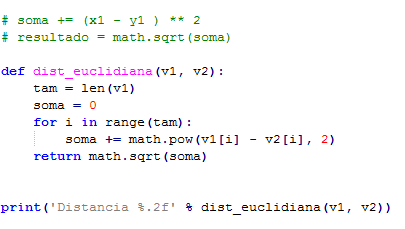
\includegraphics[scale=1, keepaspectratio]{figuras/codigodistanciaeuclidianaempython}
		\label{dist_eu_py}
	%\fonte{\cite{fayyad1996data}}
\end{figure}

\begin{figure}[h]
	\caption{\textbf{Exemplo de Distância Euclidiana em \emph{Python} com biblioteca \emph{Numpy}}}
	\centering
		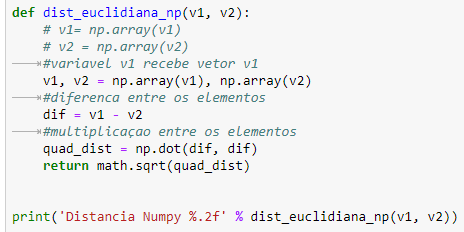
\includegraphics[scale=1, keepaspectratio]{figuras/codigodistanciaeuclidianaempythonnumpy}
		\label{dist_eu_pynumpy}
	%\fonte{\cite{fayyad1996data}}
\end{figure}

\par Como é visto  nas figuras \ref{dist_eu_py} e na figura \ref{dist_eu_pynumpy},aplicações de funções da Distância Euclidiana em \emph{Python}, sendo que na figura \ref{dist_eu_pynumpy} foi aplicada a formula da Distância Euclidiana com auxilio da biblioteca \emph{Numpy}, notando se que as variáveis v1 e v2 são vetores que recebem listas com uma amostragem de dados, nesse caso uma série de números variados, após isso é feito a diferença nas variáveis que na verdade são matrizes, e depois é realizada a multiplicação entre as matrizes e depois é retornada a raiz quadrada das matrizes, e é verificado o cálculo obtendo o resultado que tende a ser o mais próximo de zero, para poder demostrar um agrupamento de padrões nos dados.



% ---

% ---
% Incluindo Capitulo 4 - Casos de Testes
\newpage
\chapter{RESULTADOS}

\par Neste capítulo serão apresentados os resultados e análises obtidos nos estudos dos dados. E para verificação dos algoritmos e dos dados o arquivo encontra-se no \emph{site} \emph{Github} no \emph{link}: https://github.com/nata27junior/Dataframe-Tg-dados.



\section{Resultados obtidos com Distância Euclidiana}
\par Com as funções descritas nas figuras \ref{dist_eu_py} e \ref{dist_eu_pynumpy}, e aplicando-as  nos dados  foram obtidos os seguintes resultados:

\begin{figure}[ht]
	\caption{\textbf{Aplicação Distância Euclidiana nos meses de Março e Abril de 2018}}
	\centering
		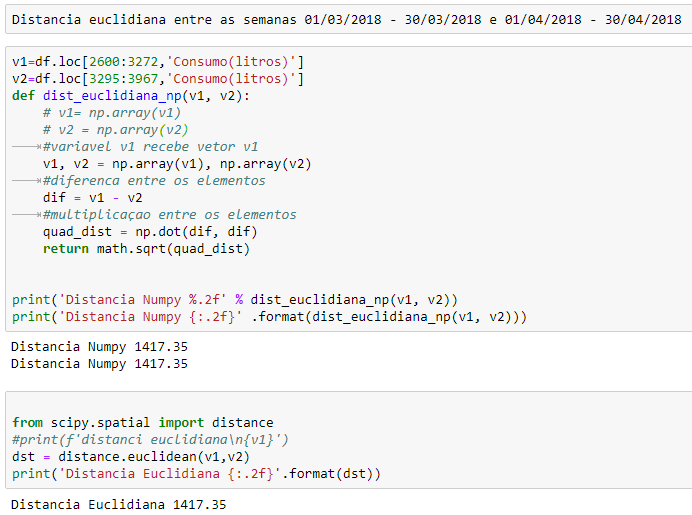
\includegraphics[width=\textwidth,height=\textheight , keepaspectratio]{figuras/distanciaeuclidiana01-03-2018-30-03-2018-01-04-18-30-04-18}
		\label{dist_Marco_Abril}
	%\fonte{\cite{fayyad1996data}}
\end{figure}
\par Com as funções de Distância Euclidiana, aplicadas nos dados relativos há dois meses, março de 2018 e abril de 2018, foi obtido o seguinte resultado de  $\approx$ 1417, observa-se isso na figura \ref{dist_Marco_Abril}.  Relembrando que distância euclidiana é uma das medidas de dissimilaridade entre comunidades mais utilizadas na prática. E quanto menor o valor da distância euclidiana entre os dados, mais próximos os pontos se apresentam, logo, quanto menor a distância entre os pontos, maior a eficiência do procedimento.

\begin{figure}[ht]
	\caption{\textbf{Gráfico de comparação dos meses de março e abril de 2018 com a Distância Euclidiana}}
	\centering
		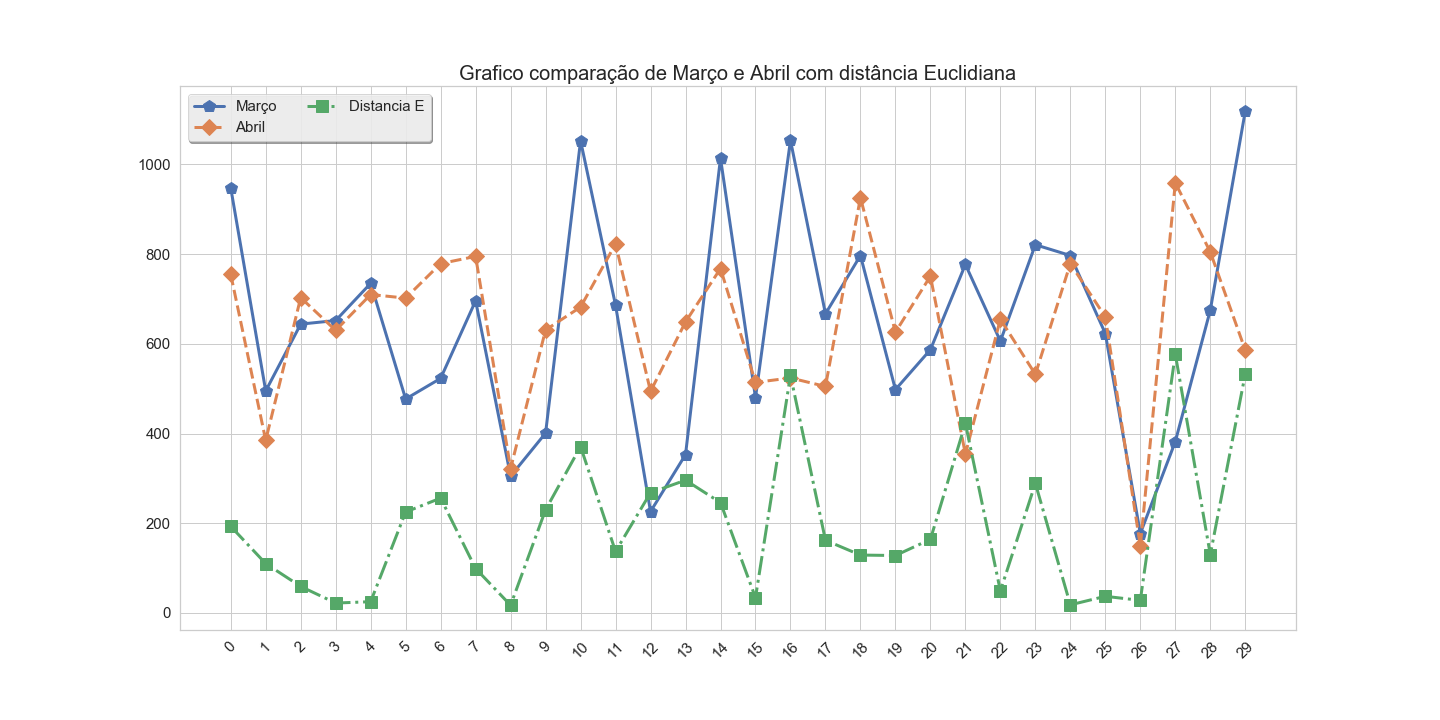
\includegraphics[width=\textwidth,height=\textheight , keepaspectratio]{figuras/ComparacaodeMarcoeAbrilcomdistanciaEuclidiana}
		\label{graf_dist_Marco_Abril}
	%\fonte{\cite{fayyad1996data}}
\end{figure}
\par Nesse gráfico, da figura \ref{graf_dist_Marco_Abril}, foi aplicada a função da Distância Euclidiana no consumo diário nos meses de março e abril de 2018, aplicada ponto a ponto, e notando se que em alguns dias o consumo diário dos meses foi quase semelhante onde os resultados da função da Distância Euclidiana quase se aproxima a zero. 

\begin{figure}[ht]
	\caption{\textbf{Aplicação da Distancia Euclidiana entre duas semanas setembro de 2017}}
	\centering
		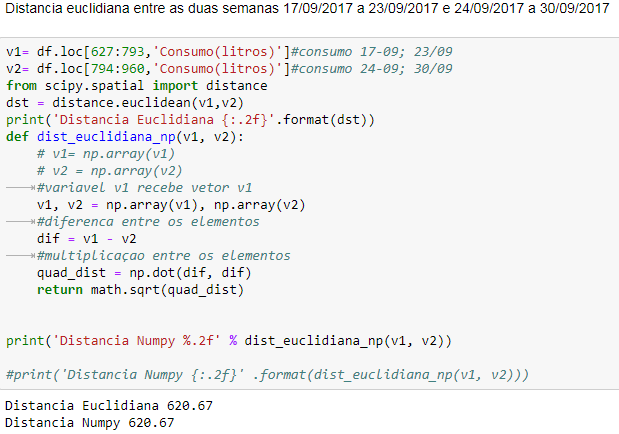
\includegraphics[width=\textwidth,height=\textheight , keepaspectratio]{figuras/distanciaeuclidiana17-09a23-09e24-09a30-09}
		\label{dist_duas_set}
	%\fonte{\cite{fayyad1996data}}
\end{figure}

\par Executando as funções de Distância Euclidiana entre duas semanas, de 17 de setembro a 23 de setembro e 24 de setembro a 30 de setembro, obteve-se o resultado de  $\approx$ 620. Mas uma vez, o resultado obtido não foi mais próximo de zero, como se observa na figura  \ref{dist_duas_set}.

\begin{figure}[ht]
	\caption{\textbf{Gráfico de comparação entre duas semanas com a Distância Euclidiana}}
	\centering
		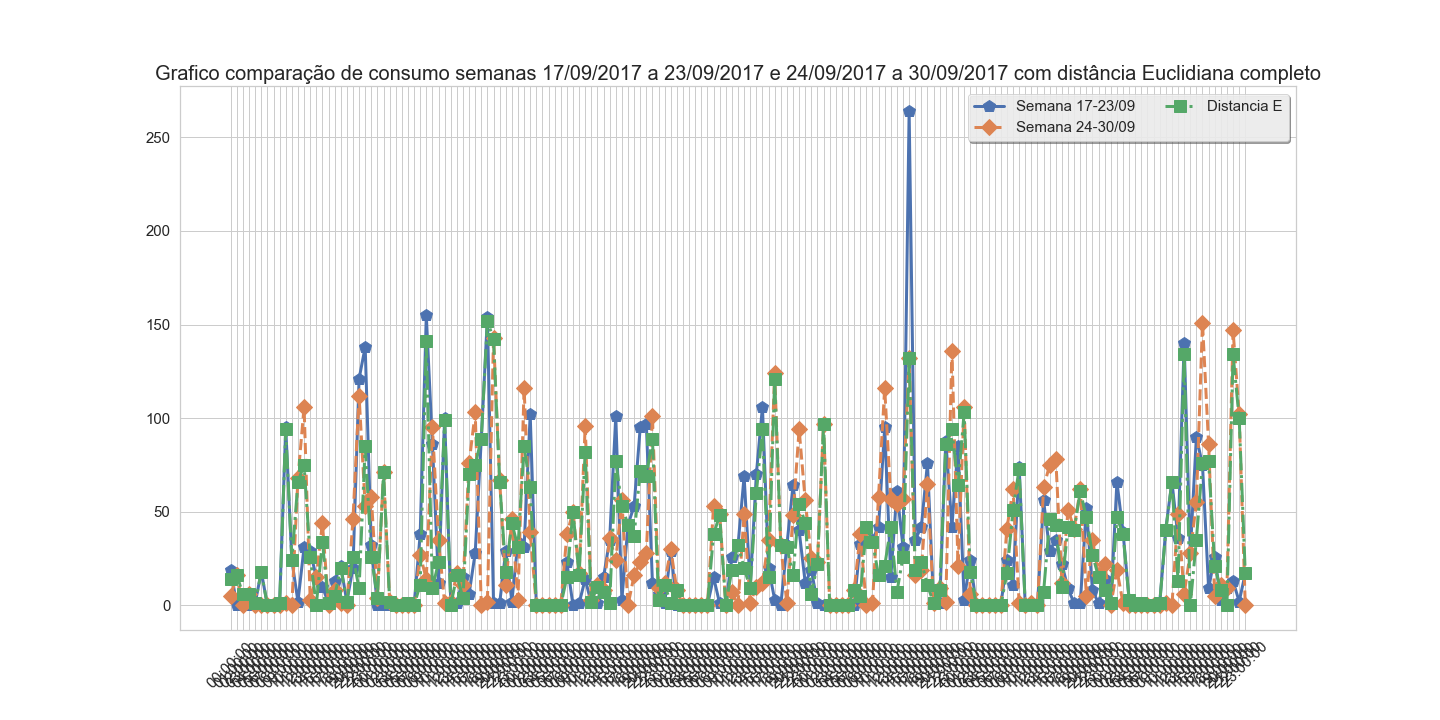
\includegraphics[width=\textwidth,height=\textheight , keepaspectratio]{figuras/Comparacaodesemanas17a23-09e24a30-09comdistanciacompleto}
		\label{dist_duas_set_comp}
	%\fonte{\cite{fayyad1996data}}
\end{figure}

\begin{figure}[ht]
	\caption{\textbf{Gráfico de comparação entre duas semanas com a Distância Euclidianas Detalhadas}}
	\centering
		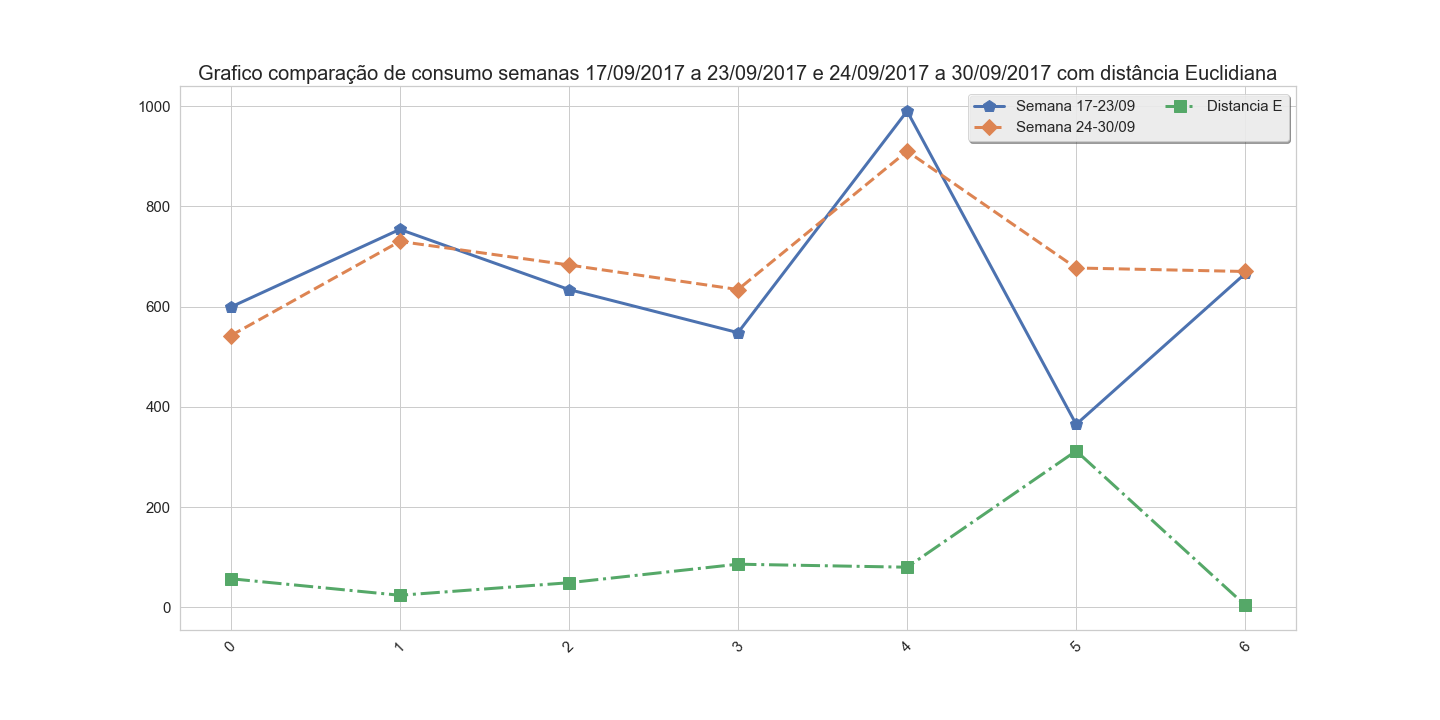
\includegraphics[width=\textwidth,height=\textheight , keepaspectratio]{figuras/Comparacaodesemanas17a23-09e24a30-09comdistancia}
		\label{dist_duas_set_deta}
	%\fonte{\cite{fayyad1996data}}
\end{figure}

\par No gráfico da figura \ref{dist_duas_set_comp} representa o consumo entre duas semanas de 17 de setembro a 23 de setembro e 24 de setembro a 30 de setembro, com a distância euclidiana aplicada ponto a ponto, mesmo com o gráfico com  os dados muito próximo pode verificar que há pontos onde o resultado da função aproximou de zero . E pode conferir com mais detalhes no gráfico da figura \ref{dist_duas_set_deta}, onde foi aplicada a função no consumo diário, observando que o consumo nos dias foram bem semelhante e o resultado da função foi bem próximo de zero. 

\begin{figure}[ht]
	\caption{\textbf{Aplicação da Distancia Euclidiana entre os dias 09 e 16 de setembro de 2017}}
	\centering
		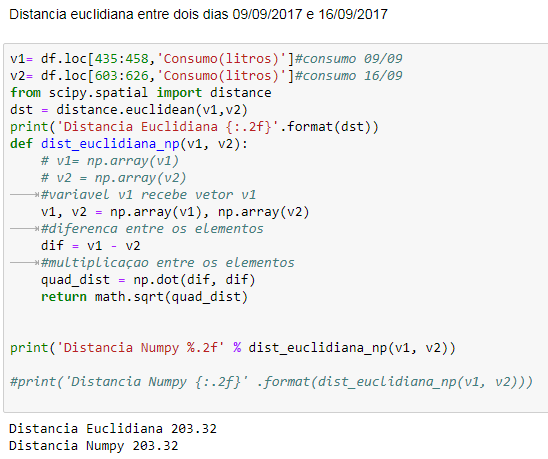
\includegraphics[scale=0.8 , keepaspectratio]{figuras/distanciaeuclidiana09-09-17e16-09-17}
		\label{dist_09e16_set_deta}
	%\fonte{\cite{fayyad1996data}}
\end{figure}

\par Executando as funções de Distância Euclidiana em dois dias, 09 e 16, do mês de setembro, dois sábados do mesmo mês, e obteve-se o resultado de  $\approx $203. Mas uma vez, o resultado obtido não sendo mais próximo de zero (0), como se observa na figura \ref{dist_09e16_set_deta}. 

\begin{figure}[ht]
	\caption{\textbf{Gráfico de comparação entre os dias 09 e 16 de setembro de 2017 com Distância Euclidiana}}
	\centering
		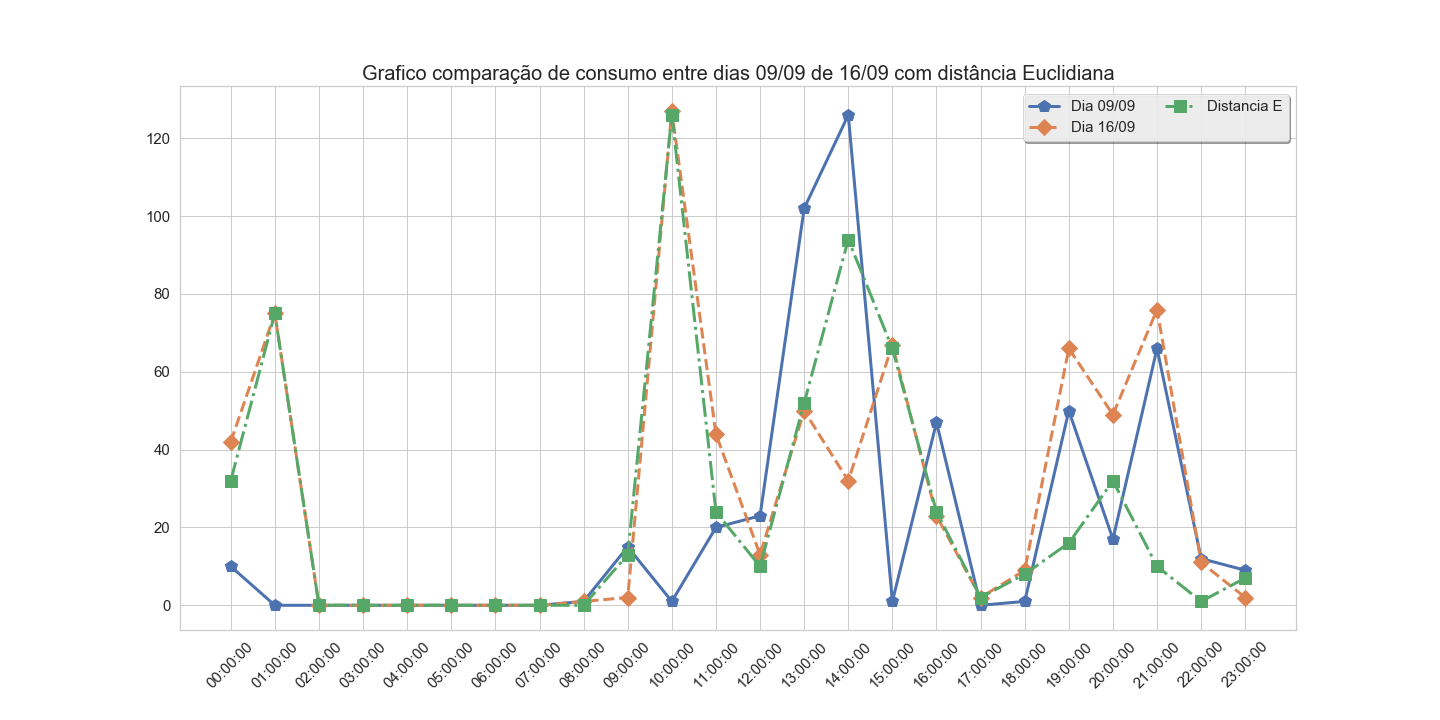
\includegraphics[width=\textwidth,height=\textheight , keepaspectratio]{figuras/Comparacaodedias09-09e16-09comdistancia}
		\label{graf_dist_09e16_set_deta}
	%\fonte{\cite{fayyad1996data}}
\end{figure}
\par O Gráfico da figura \ref{graf_dist_09e16_set_deta} representa o consumo entre dois dias, 09 de setembro e 16 de setembro, dois sábados do mesmo mês,  aplicada a função da Distância ponto a ponto, observa que no período onde não houve consumo os resultados foram próximos a zero, e em alguns pontos onde teve consumo o resultado da função também se aproximou de zero sendo um comportamento do consumo muito parecido.


\section{Resultados obtidos com a Função para plotagem de gráfico }
\par Com a função de plotagem de gráfico que foi discriminar na figura \ref{codigo_plotagem}, podemos verificar as seguintes situações. 

\begin{figure}[ht]
	\caption{\textbf{Gráfico de comparação entre Domingos}}
	\centering
		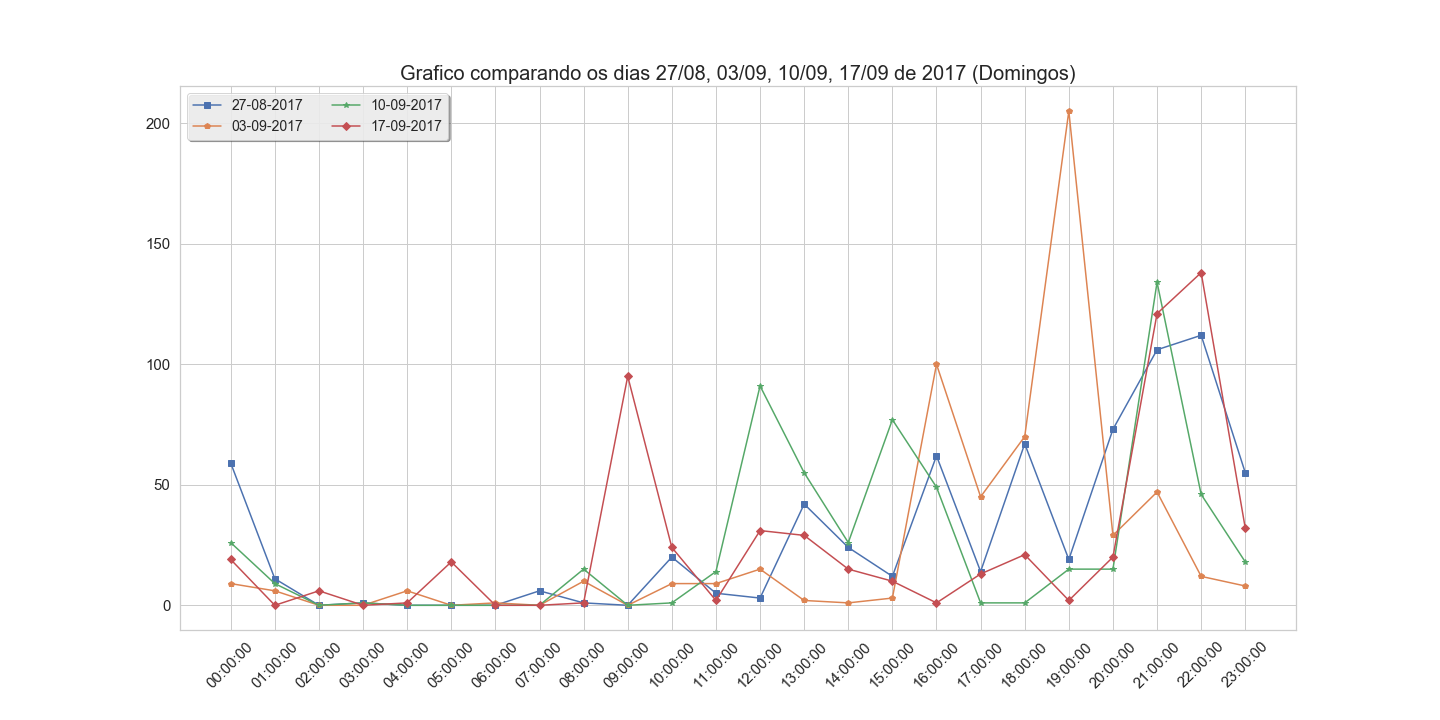
\includegraphics[width=\textwidth,height=\textheight , keepaspectratio]{figuras/Graficocomparandoosdias27-08,03-09,10-09,17-09de2017(Domingos)}
		\label{graf_dom}
	%\fonte{\cite{fayyad1996data}}
\end{figure}

\par No gráfico da figura \ref{graf_dom}, é possível comparar os dados das seguintes datas, 27/08/2017, 03/09/2017, 10/09/2017, 17/09/2017, que são Domingos, primeiramente é observado que há um consumo semelhante entre os dias. Mas nos períodos da madrugada há um baixo consumo de água onde pode verificar  que não há vazamentos. E onde ocorrem os picos de consumo que observando mas a fundo pode se afirmar que não é um vazamentos, pois se fosse vazamento o consumo seria mais constante.  

\begin{figure}[ht]
	\caption{\textbf{Gráfico de comparação entre Segundas-Feiras}}
	\centering
		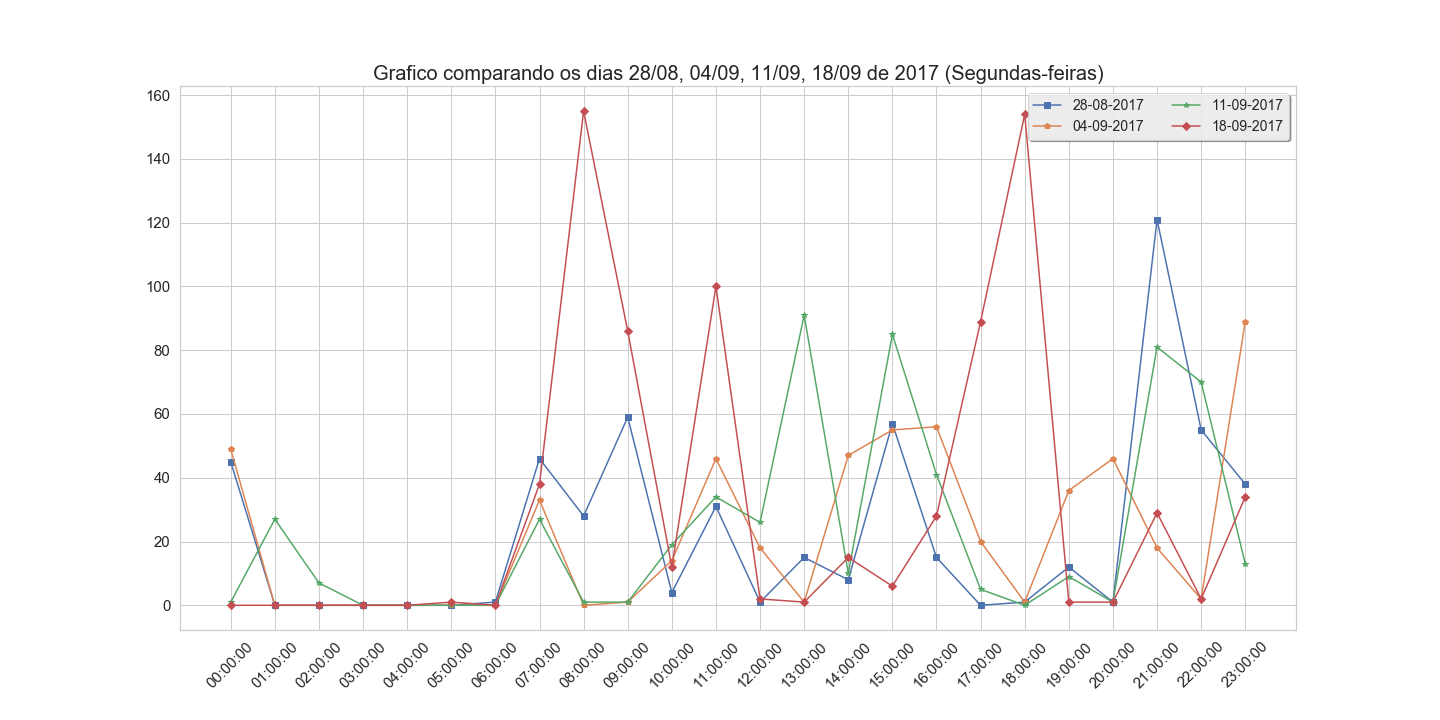
\includegraphics[width=\textwidth,height=\textheight , keepaspectratio]{figuras/Graficocomparandoosdias28-08,04-09,11-09,18-09de2017(Segundas-feiras)}
		\label{graf_seg}
	%\fonte{\cite{fayyad1996data}}
\end{figure}

\par No gráfico da figura \ref{graf_seg}, foi aplicada a função de plotagem com os dados das datas, 28/08/2017, 04/09/2017, 11/09/2017, 18/09/2017, que são segundas-feiras, obteve essa comparação dos dados, e que há um consumo semelhante.Mas nos períodos da madrugada há um baixo consumo de água onde pode verificar  que não há vazamentos. E onde ocorrem os picos de consumo que observando mas a fundo pode se afirmar que não é um vazamentos, pois se fosse vazamento o consumo seria mais constante.    

\begin{figure}[ht]
	\caption{\textbf{Gráfico de comparação entre Terças-Feiras}}
	\centering
		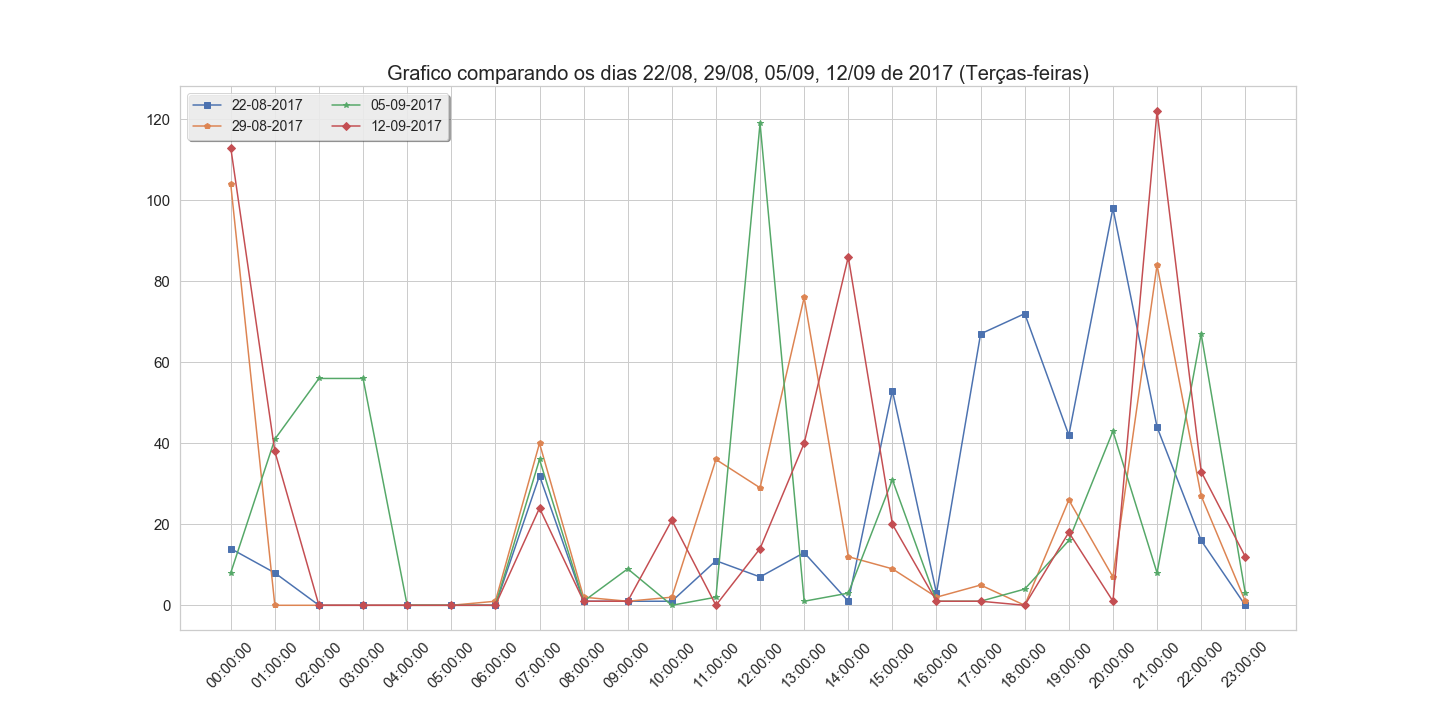
\includegraphics[width=\textwidth,height=\textheight , keepaspectratio]{figuras/Graficocomparandoosdias22-08,29-08,05-09,12-09de2017(Tercas-feiras)}
		\label{graf_ter}
	%\fonte{\cite{fayyad1996data}}
\end{figure}

\par No gráfico da figura \ref{graf_ter}, foi aplicada a função de plotagem com os dados das datas, 22/08/2017, 29/08/2017, 05/09/2017, 12/09/2017, que são terças-feiras, obteve essa comparação dos dados, e que há um consumo semelhante. Mas nos períodos da madrugada há um baixo consumo de água onde pode verificar  que não há vazamentos. E onde ocorrem os picos de consumo que observando mas a fundo pode se afirmar que não é um vazamentos, pois se fosse vazamento o consumo seria mais constante.   

\begin{figure}[ht]
	\caption{\textbf{Gráfico de Comparação dos dados entre Quartas-feiras}}
	\centering
		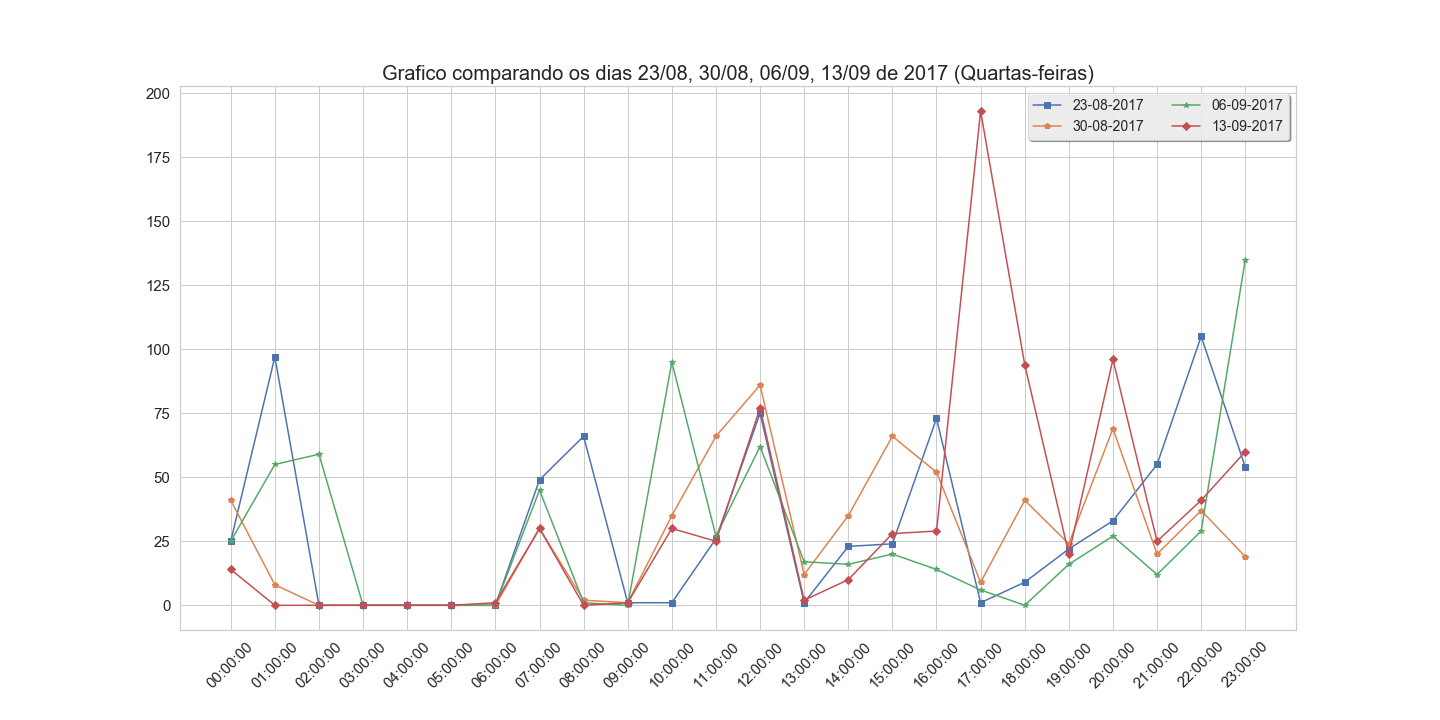
\includegraphics[width=\textwidth,height=\textheight , keepaspectratio]{figuras/Graficocomparandoosdias23-08,30-08,06-09,13-09de2017(Quartas-feiras)}
		\label{graf_quar}
	%\fonte{\cite{fayyad1996data}}
\end{figure}
\par No gráfico da figura \ref{graf_quar}, foi aplicada a função de plotagem com os dados das datas, 23/08/2017, 30/08/2017, 06/09/2017, 13/09/2017, que são quartas-feiras, obteve essa comparação dos dados, nota-se e que há um consumo semelhante. Mas nos períodos da madrugada há um baixo consumo de água onde se pode notar que não há vazamentos. E onde ocorrem os picos de consumo que observando, mas a fundo pode se afirmar que nesses picos não é um vazamentos, pois se fosse vazamento o consumo seria mais constante.  
%\begin{figure}[htb]
\begin{figure}[ht]
	\caption{\textbf{Gráfico de Comparação dos dados entre Quintas-feiras}}
	\centering
		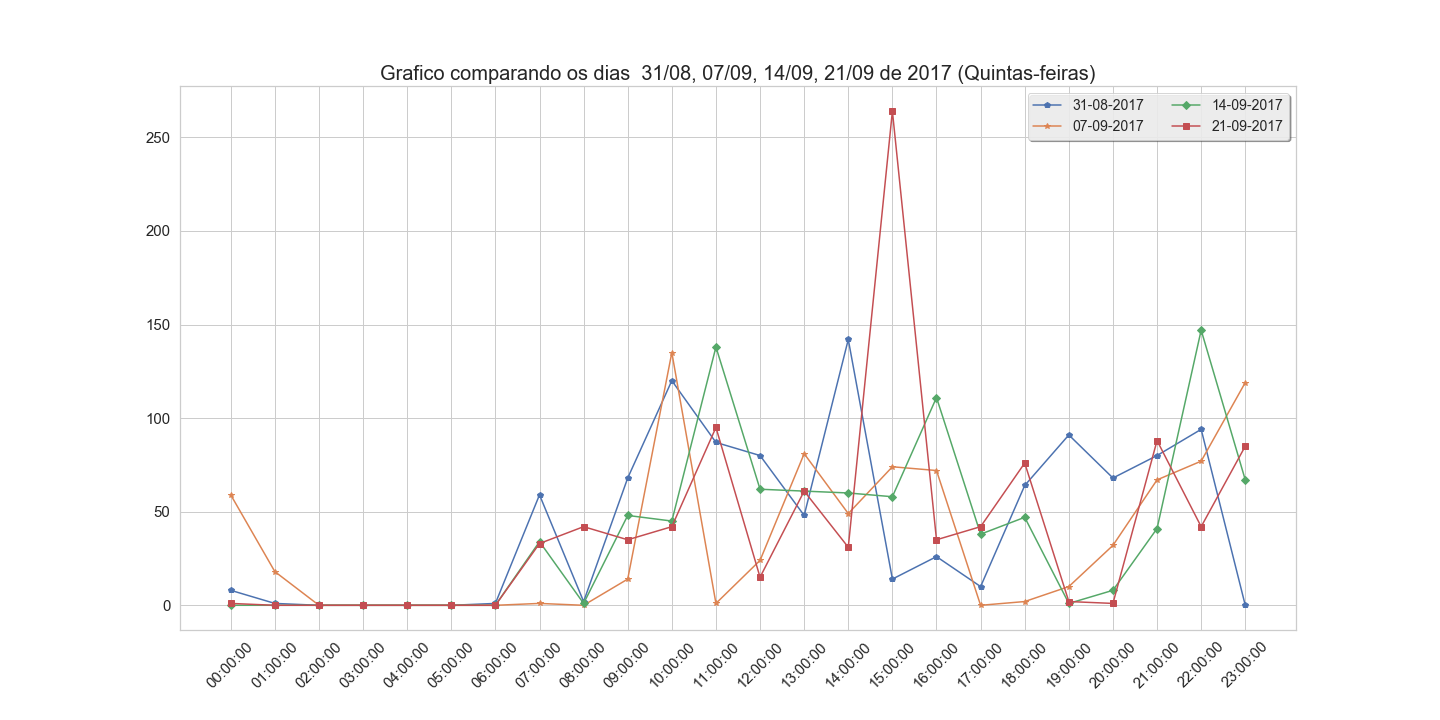
\includegraphics[width=\textwidth,height=\textheight , keepaspectratio]{figuras/Graficocomparandoosdias31-08,07-09,14-09,21-09de2017(Quintas-feiras)}
		\label{graf_qui}
	%\fonte{\cite{fayyad1996data}}
\end{figure}

\par No gráfico da figura \ref{graf_qui}, foi aplicada a função de plotagem com os dados das datas, 31/08/2017, 07/09/2017, 14/09/2017, 21/09/2017, que são quintas-feiras, obteve essa comparação dos dados, nota-se que há um consumo semelhante. Mas nos períodos da madrugada há um baixo consumo de água onde se pode notar que não há vazamentos. E onde ocorrem os picos de consumo que observando, mas a fundo pode se afirmar que nesses picos não é um vazamentos, pois se fosse vazamento o consumo seria mais constante.  

\begin{figure}[ht]
	\caption{\textbf{Gráfico de Comparação dos dados entre Sextas-feiras}}
	\centering
		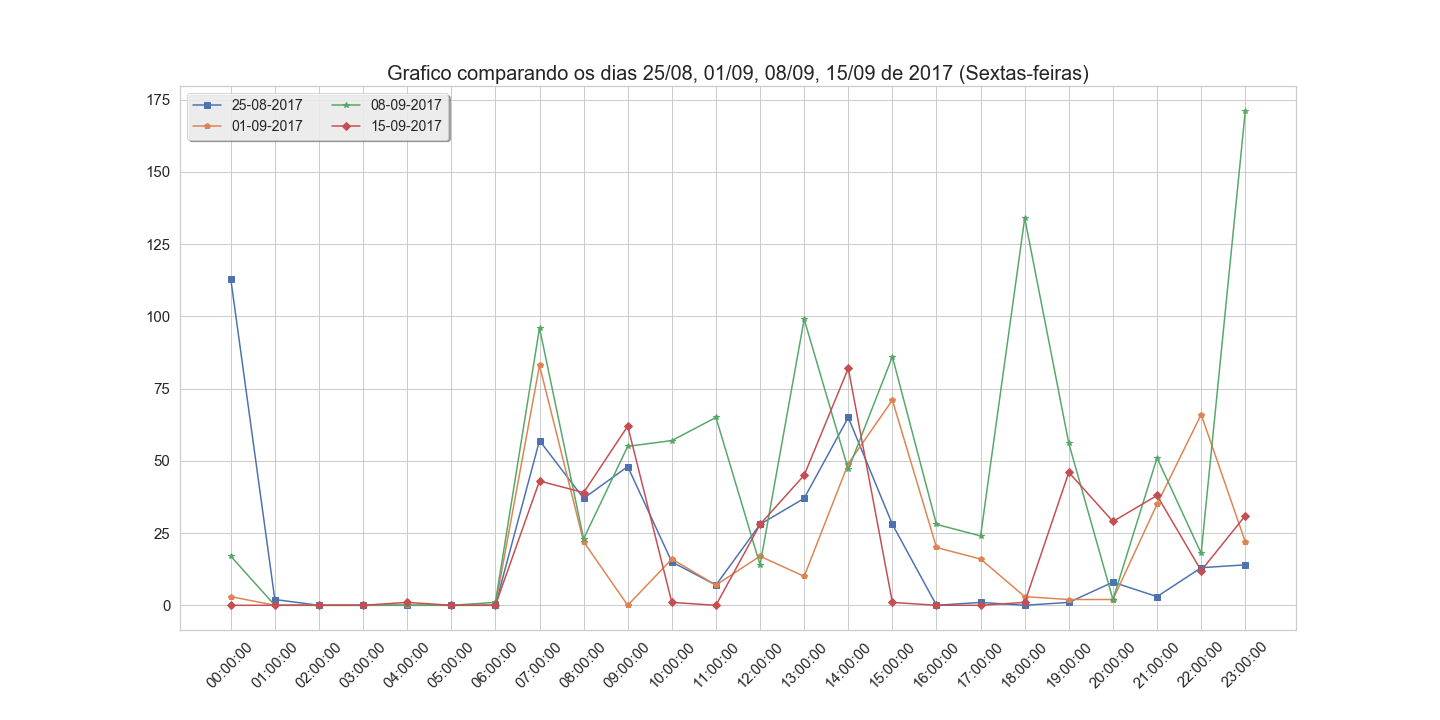
\includegraphics[width=\textwidth,height=\textheight , keepaspectratio]{figuras/Graficocomparandoosdias25-08,01-09,08-09,15-09de2017(Sextas-feiras)}
		\label{graf_sex}
	%\fonte{\cite{fayyad1996data}}
\end{figure}
\par No gráfico da figura \ref{graf_sex}, foi aplicada a função de plotagem com os dados das datas de 31/08, 07/09, 14/09 e 21/09/2017, que são sextas-feiras, obteve essa comparação dos dados, nota-se e que há um consumo semelhante. Mas nos períodos da madrugada há um baixo consumo de água onde se pode notar que não há vazamentos. E onde ocorrem os picos de consumo que observando, mas a fundo pode se afirmar que nesses picos não é um vazamentos, pois se fosse vazamento o consumo seria mais constante.  

\begin{figure}[ht]
	\caption{\textbf{Gráfico de Comparação dos dados entre Sábados}}
	\centering
		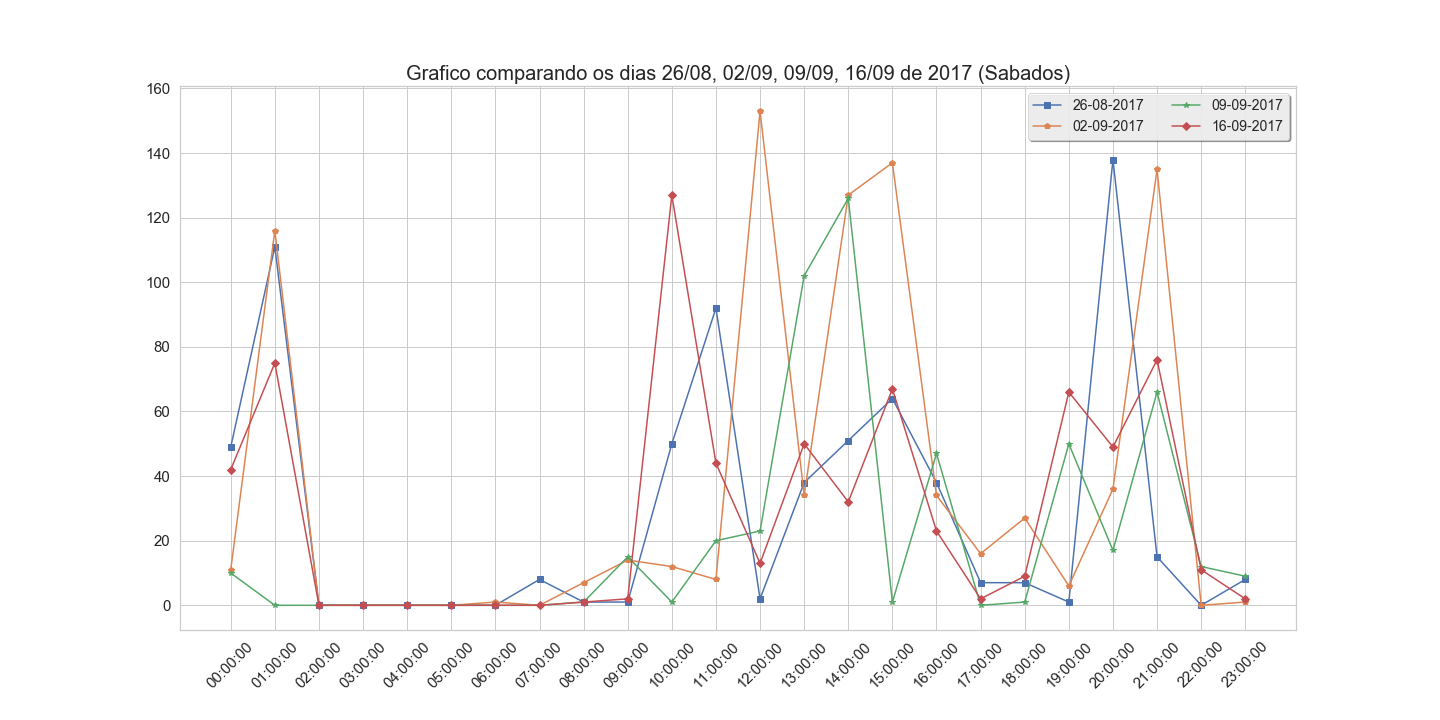
\includegraphics[width=\textwidth,height=\textheight , keepaspectratio]{figuras/Graficocomparandoosdias26-08,02-09,09-09,16-09de2017(Sabados)}
		\label{graf_sab}
	%\fonte{\cite{fayyad1996data}}
\end{figure}

\par No gráfico da figura \ref{graf_sab}, foi aplicada a função de plotagem com os dados das datas  de 26/08, 02/09, 09/09 e 16/09/2017, que são sábados, obteve essa comparação dos dados, nota-se e que há um consumo semelhante. Mas nos períodos da madrugada há um baixo consumo de água onde se pode notar que não há vazamentos. E onde ocorrem os picos de consumo que observando, mas a fundo pode se afirmar que nesses picos não é um vazamentos, pois se fosse vazamento o consumo seria mais constante.

\begin{figure}[ht]
	\caption{\textbf{Gráfico de comparação com diferença entre 03 a 09/09 e 10 a 16/09}}
	\centering
		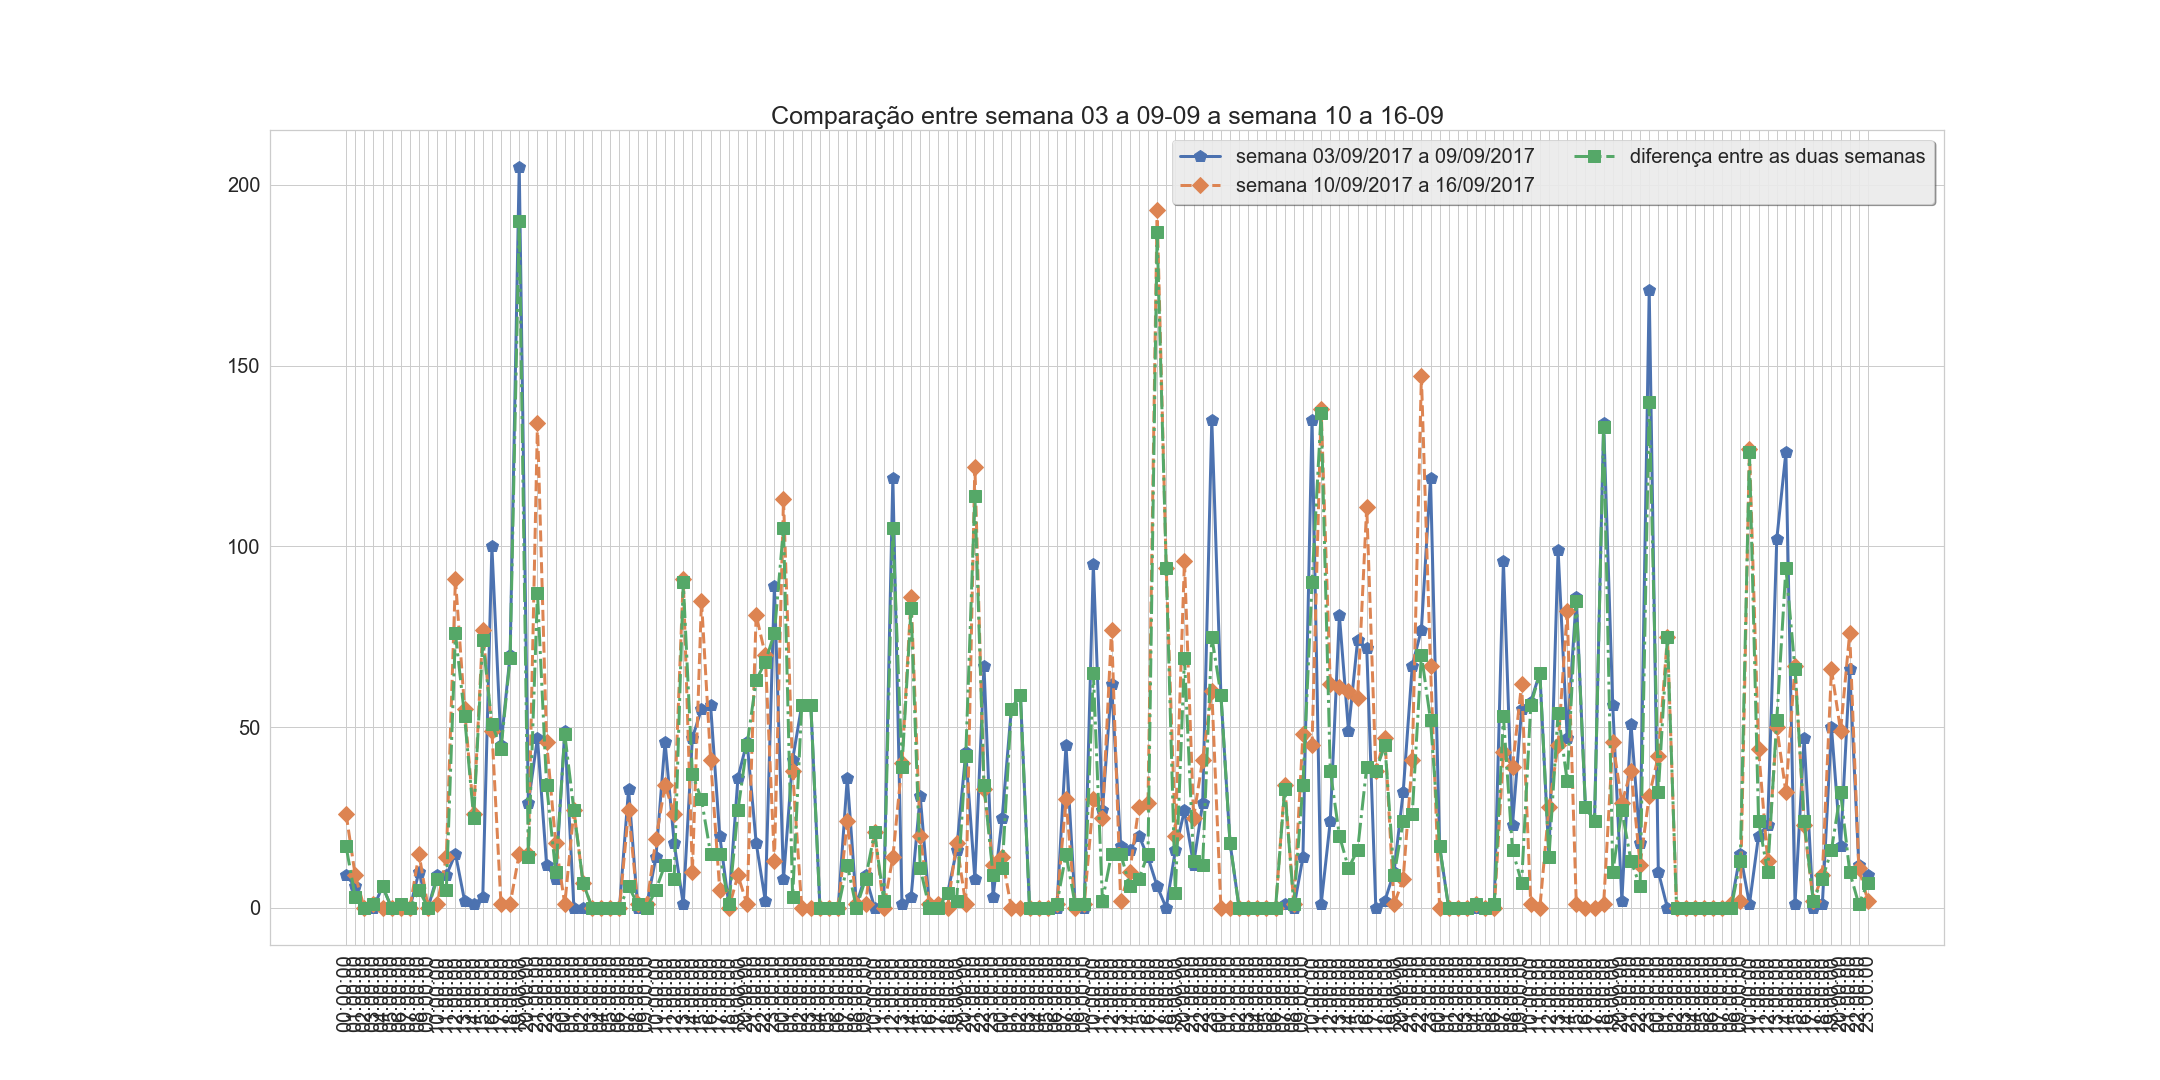
\includegraphics[width=\textwidth,height=\textheight , keepaspectratio]{figuras/comparacaoentresemana03a09-09asemana10a16-09}
		\label{graf_semana03a09}
	%\fonte{\cite{fayyad1996data}}
\end{figure}
\par Com o gráfico da figura \ref{graf_semana03a09}, trata-se da aplicação da função de plotagem fazendo uma comparação dos dados entre duas semanas. Uma semana é de 03 de setembro a 09 de setembro e outra semana é de 10 de setembro a 16 de setembro, e uma linha do gráfico se trata de diferença de consumo hora a hora entre essas duas semanas. Com os pontos muito próximos fica complicada a visualização dos pontos, mas há períodos onde não há consumo podendo afirmar que não houve vazamentos.

\begin{figure}[ht]
	\caption{\textbf{Gráfico detalha a comparação com diferença entre a 09/09 e  16/09}}
	\centering
		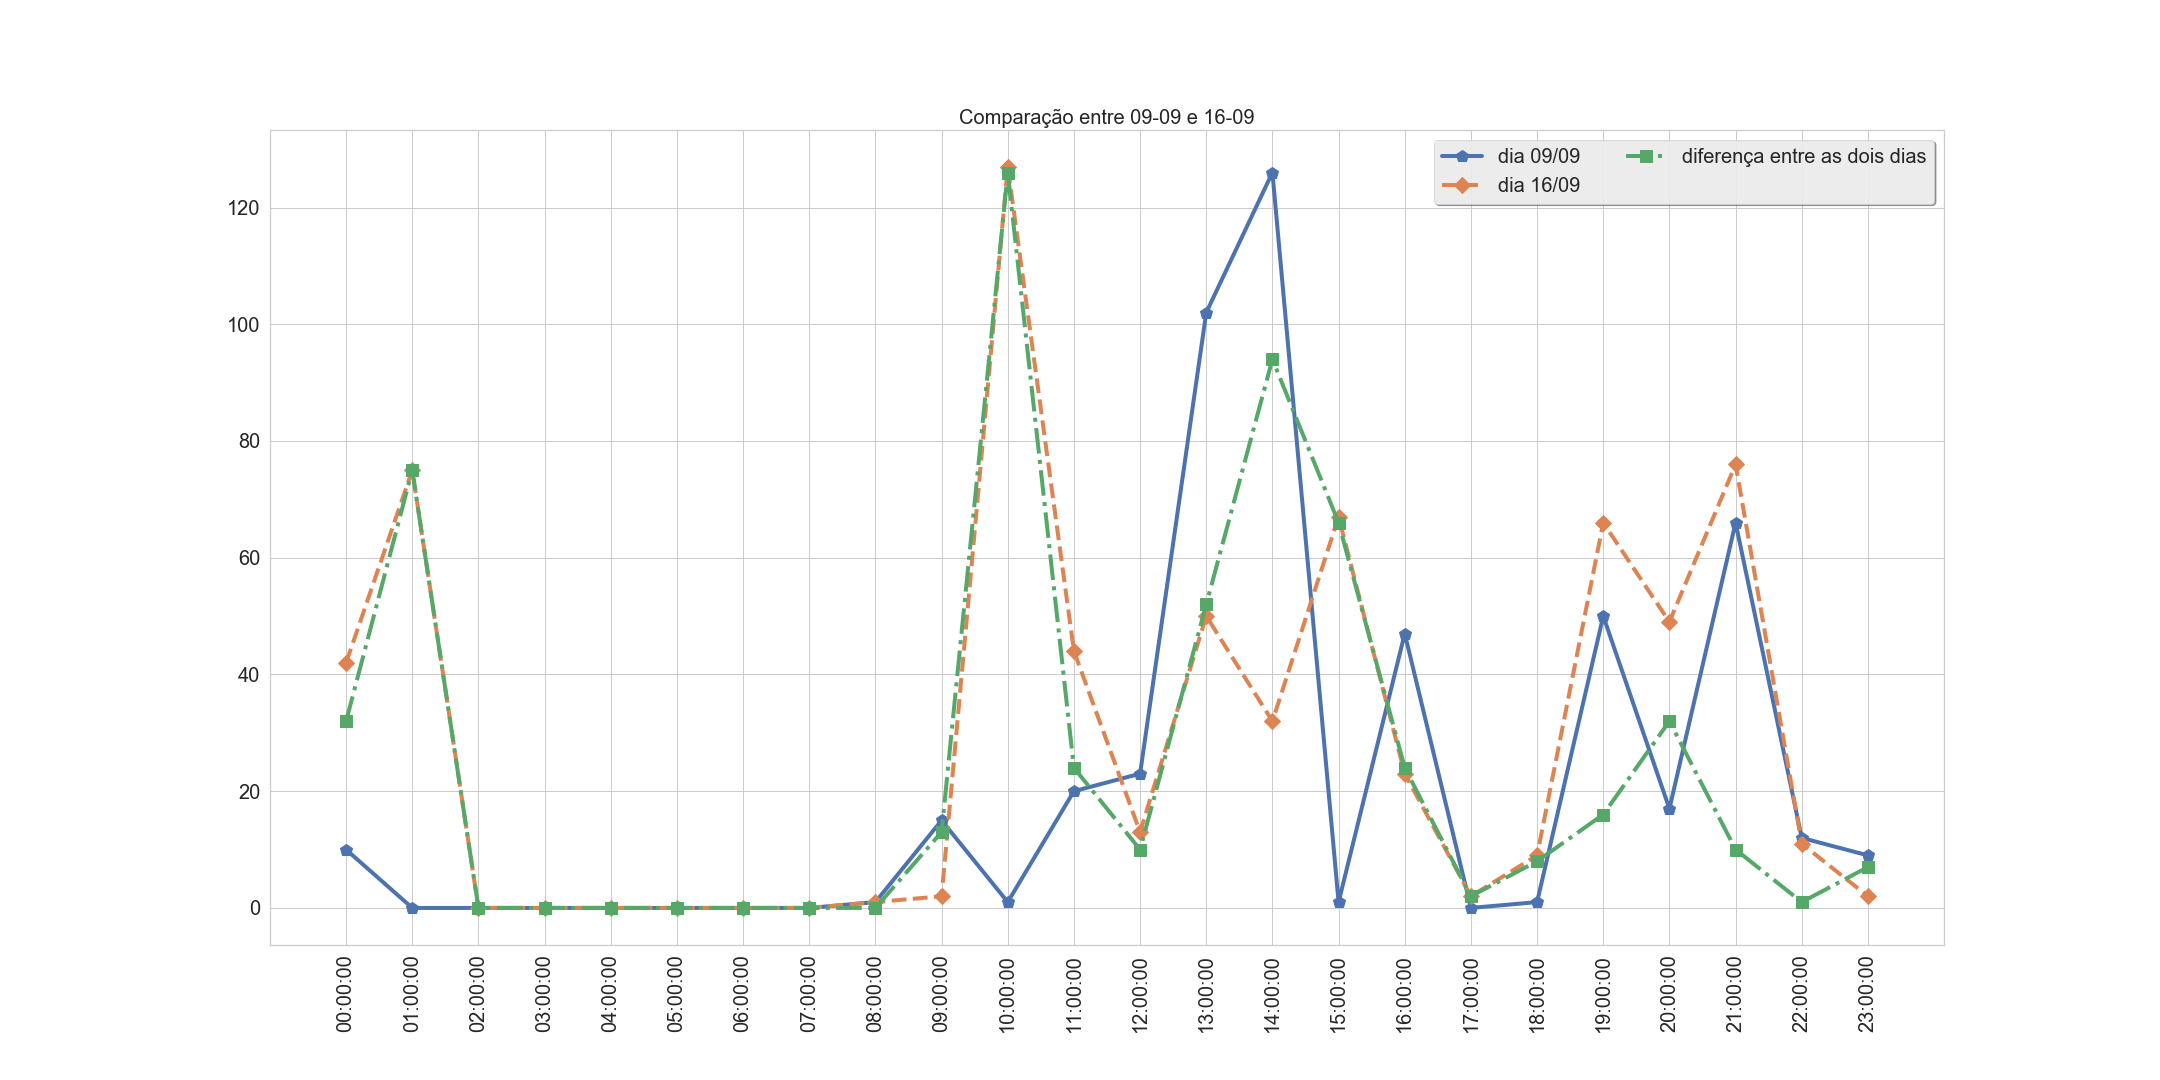
\includegraphics[width=\textwidth,height=\textheight , keepaspectratio]{figuras/zoomdacomparacaoentresemana03a09-09asemana10a16-09}
		\label{graf_det_semana03a09}
	%\fonte{\cite{fayyad1996data}}
\end{figure}
\par Com o gráfico da figura \ref{graf_det_semana03a09} trata-se da aplicação da função de plotagem nos dados fazendo uma comparação entre dois dias, com uma linha mostrando a diferença ponto a ponto, os dados utilizados para esse gráfico foi os dados dos dias 09 e 16 de setembro de 2017 e trata-se das últimas 24 horas podendo ver com mais detalhes as linhas que dos dias e a diferença dos dados. Nos horários da madrugada pode-se verificar que não há consumo de água.  

\begin{figure}[ht]
	\caption{\textbf{Figuras mostrando os dias com maior consumo de água}}
	\centering
		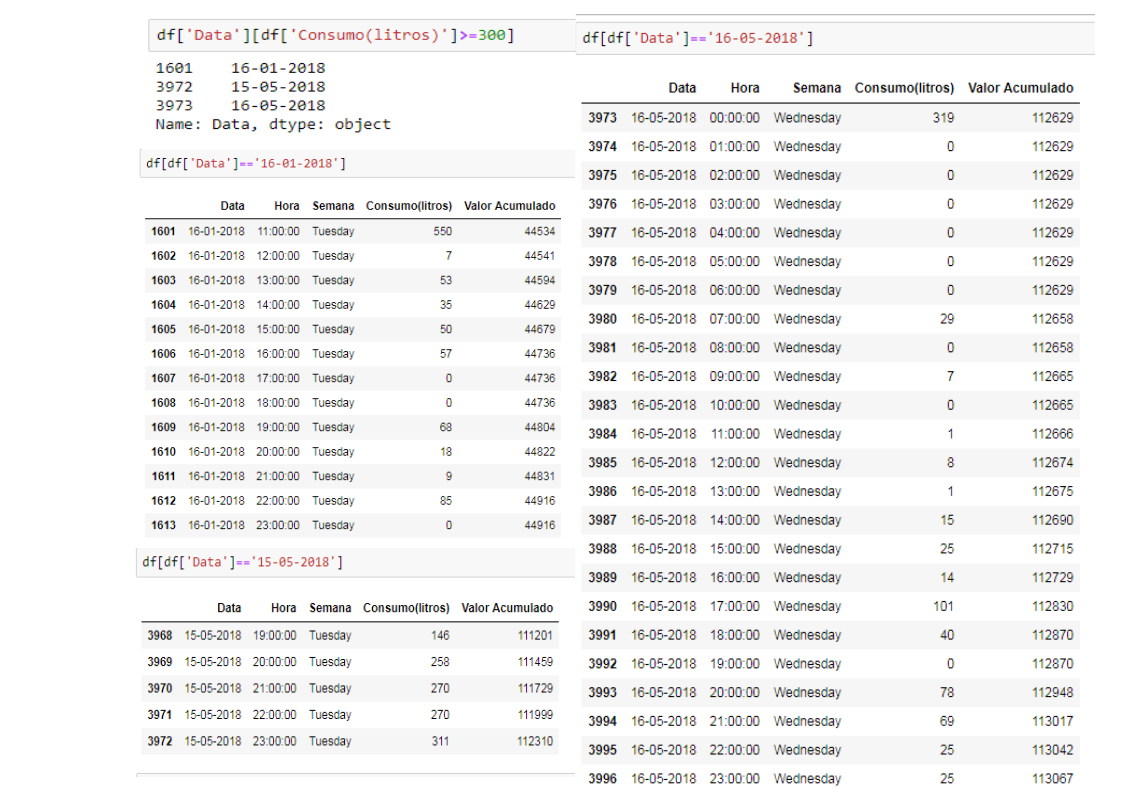
\includegraphics[width=\textwidth,height=\textheight , keepaspectratio]{figuras/datascommaiorconsumo2}
		\label{fig_maior_consumo}
	%\fonte{\cite{fayyad1996data}}
\end{figure}

\begin{figure}[ht]
	\caption{\textbf{Plotagem dos dados dos dias de maior consumo}}
	\centering
		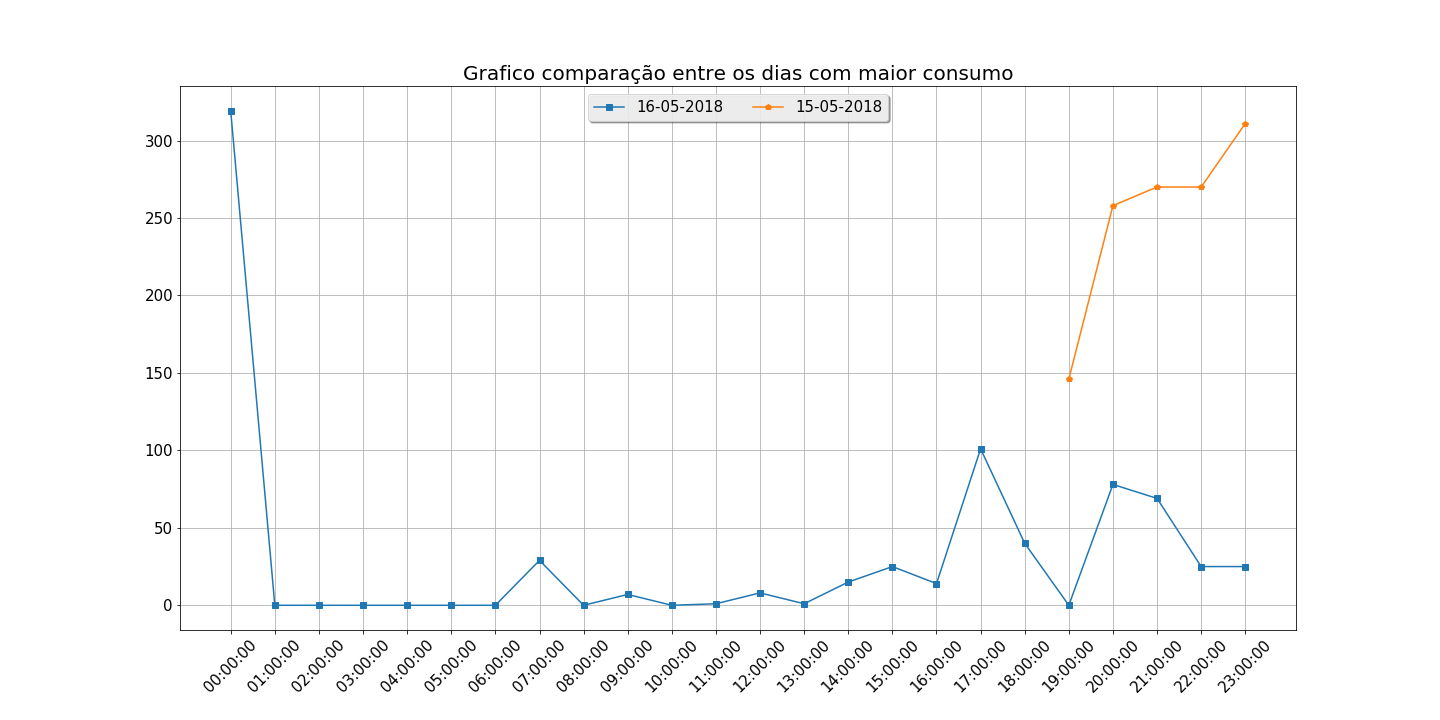
\includegraphics[width=\textwidth,height=\textheight , keepaspectratio]{figuras/comparacaoentreosdiascommaiorconsumo}
		\label{plot_maior_consumo}
	%\fonte{\cite{fayyad1996data}}
\end{figure}

\par Na figura \ref{fig_maior_consumo},  utiliza-se uma função especifica para mostrar os dias com maior consumo de água. Esses dias o consumo ultrapassa os 300 litro de água. Na figura \ref{plot_maior_consumo} uma plotagem que mostra os dias com maior consumo de água. Nota-se que no dia 15/05/2018 não tem os dados de consumo de todas as horas. O registro dos  dados é a partir das 19hs, não foi passada a informação se houve falha no equipamento para obtenção dos dados, ocasionando essa amostra com índice muito elevado de consumo. No dia 16/05/2018 há o registro de consumo após as 00hs, não se sabe se foi decorrente ao dia anterior que teve falha nos dados ou se realmente foi um consumo excessivo, mas como já observado nas horas da madrugada não há consumo de água, passa-se a ideia que no sistema não houve vazamento. O mesmo ocorre no  dia 16/01/2018 também se obteve um registro de dados elevado acima de 550 litros, como se pode notar a obtenção dos dados foi a partir das 11hs, então não se sabe se foi falha no sistema ou realmente teve um consumo elevado.

\begin{figure}[ht]
	\caption{\textbf{Gráfico com médias diárias de toda amostragem}}
	\centering
		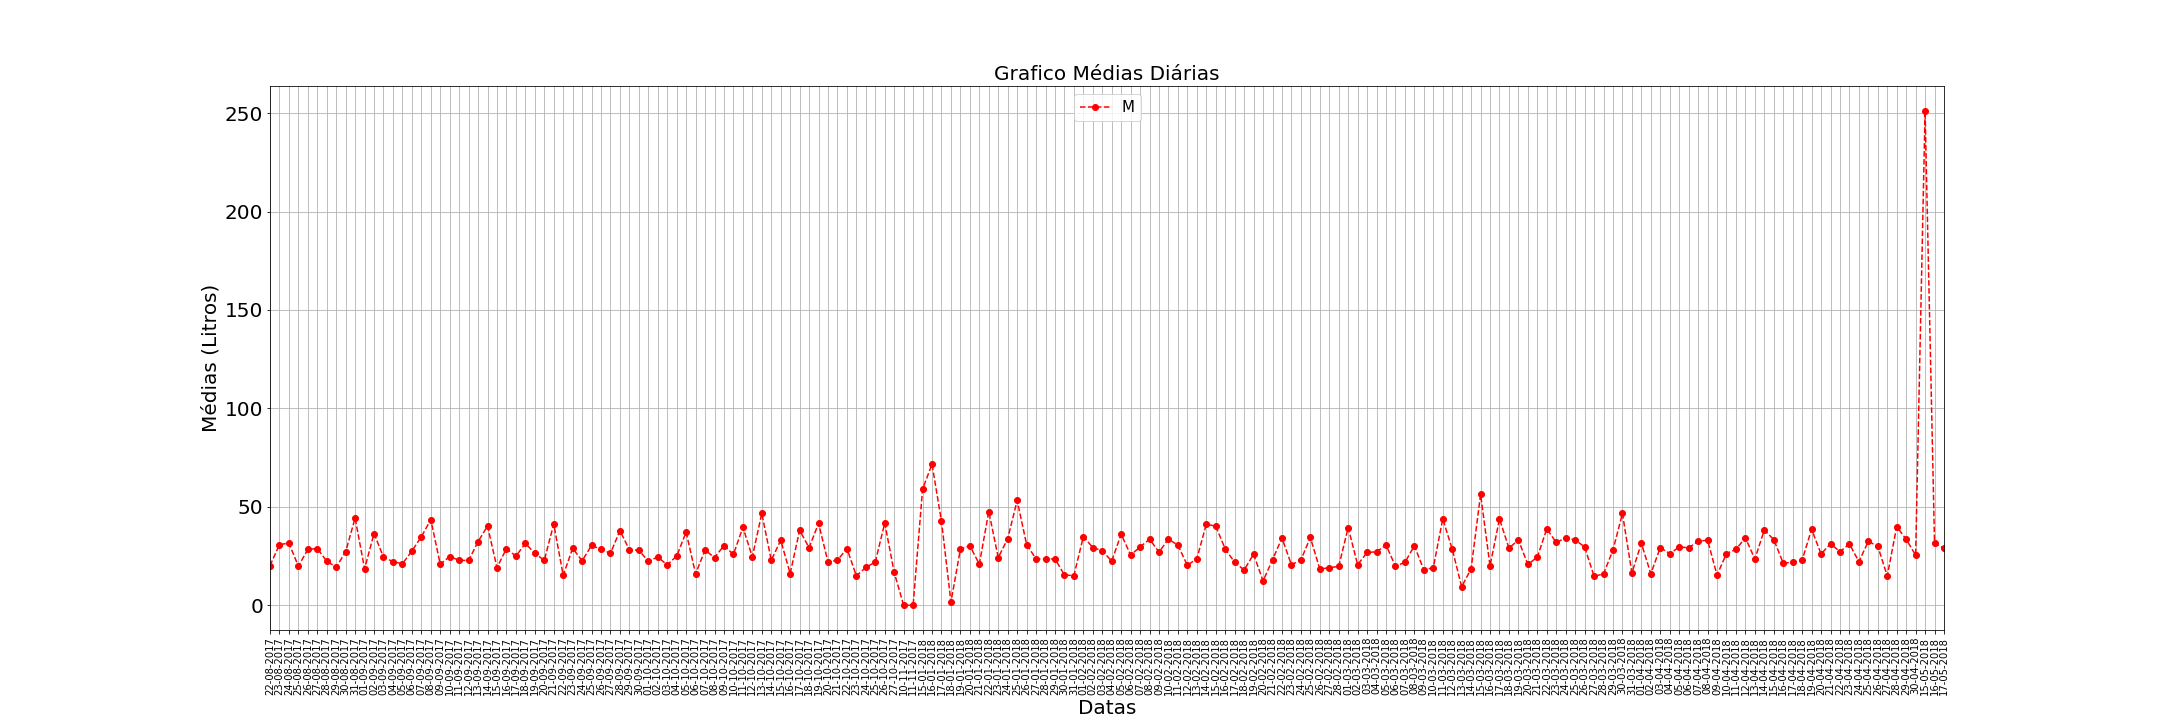
\includegraphics[width=\textwidth,height=\textheight , keepaspectratio]{figuras/GraficoMediasDiarias(este)}
		\label{graf_media_diaria}
	%\fonte{\cite{fayyad1996data}}
\end{figure}

\begin{figure}[ht]
	\caption{\textbf{Gráfico detalhado com médias diárias}}
	\centering
		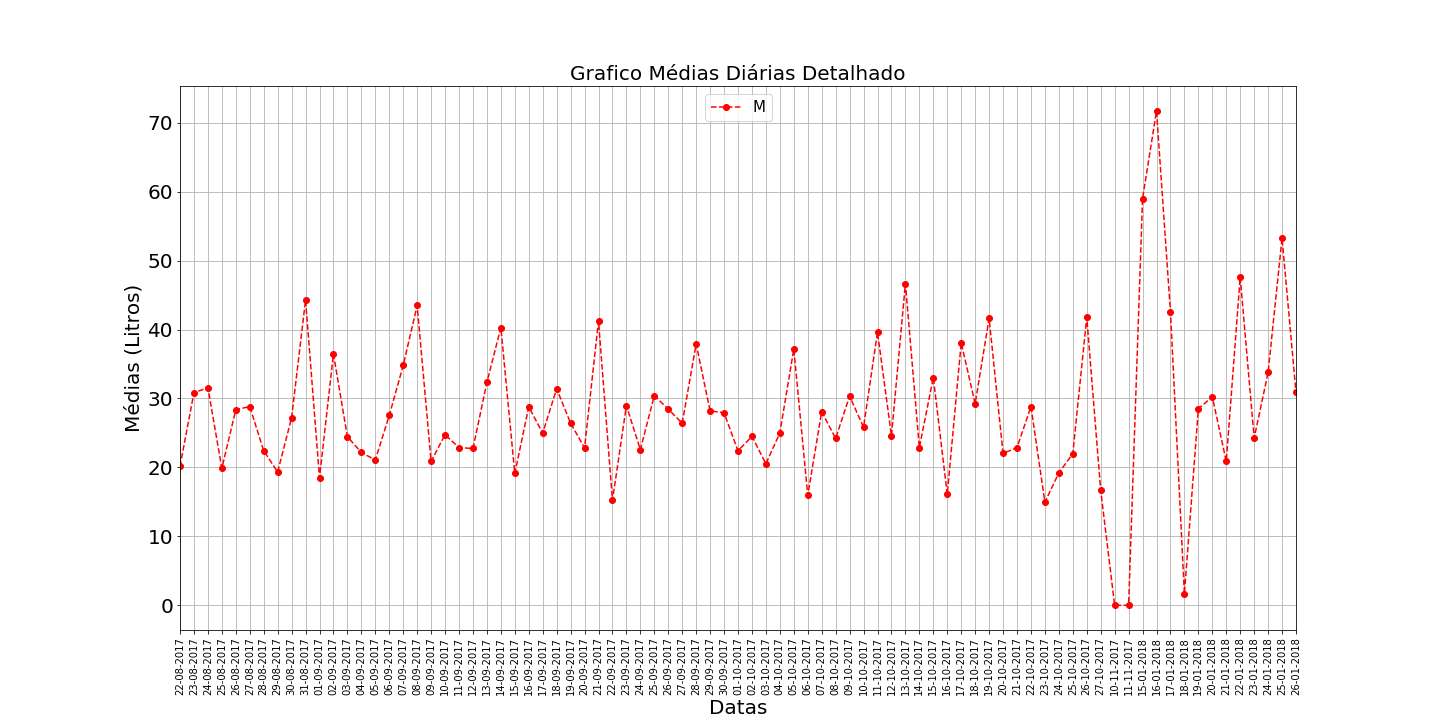
\includegraphics[width=\textwidth,height=\textheight , keepaspectratio]{figuras/GraficoMediasDiarias(estecomzoom)}
		\label{graf_media_diaria_detal}
	%\fonte{\cite{fayyad1996data}}
\end{figure}


\par Com a função detalhada na figura \ref{codigo_medias_diarias} onde foi possível realizar o cálculo das médias diárias do arquivo todo. E com a plotagem dos dados obtidos no gráfico da figura \ref{graf_media_diaria} e também no gráfico da figura \ref{graf_media_diaria_detal} sendo que este é uma plotagem dos dados mais detalhados para verificação das datas, e  observa que na maioria dos dias o consumo médio não ultrapassa 50 litros.



\begin{figure}[ht]
	\caption{\textbf{Gráfico com médias diárias dos meses setembro e outubro com Distância Euclidiana}}
	\centering
		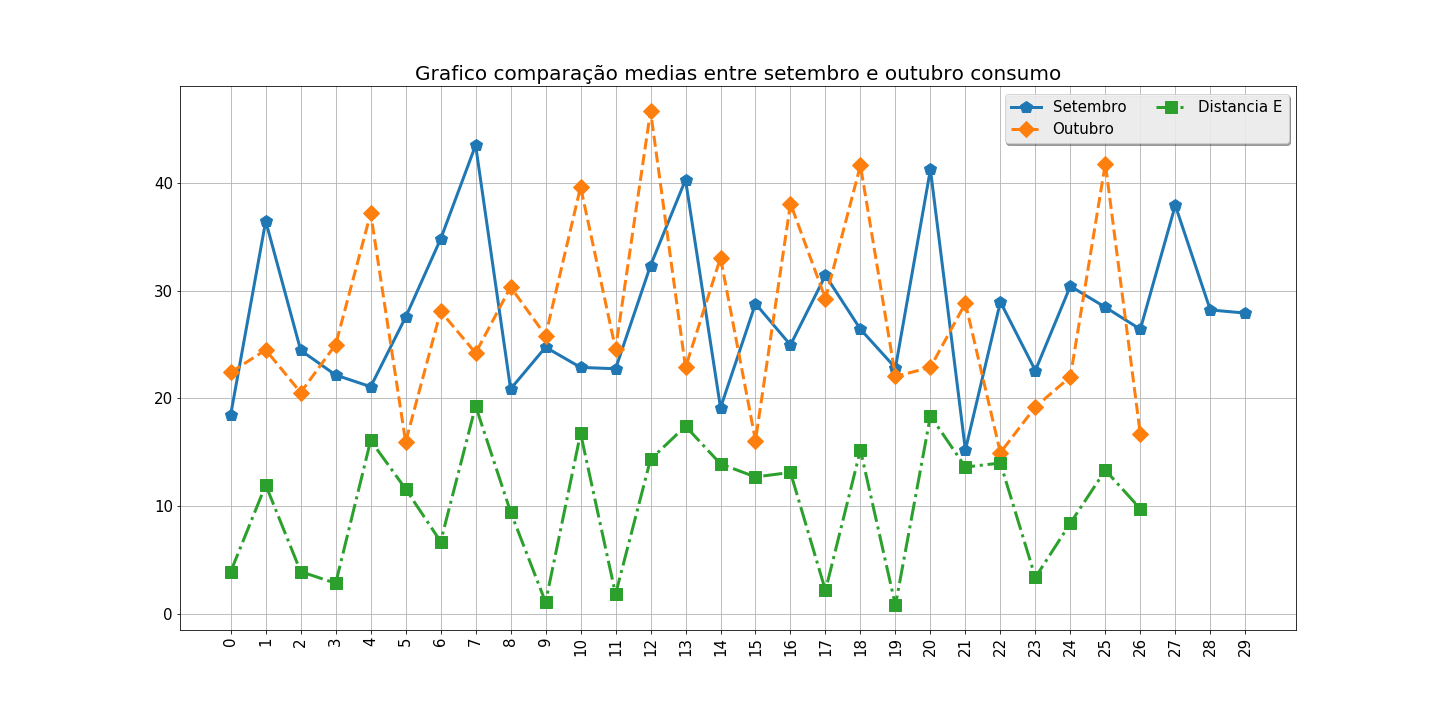
\includegraphics[width=\textwidth,height=\textheight , keepaspectratio]{figuras/comparacaomediasentredoismesesconsumocomdistanciae}
		\label{graf_media_diaria_meses_d}
	%\fonte{\cite{fayyad1996data}}
\end{figure}

\par Com o gráfico da figura \ref{graf_media_diaria_meses_d} pode se verificar a comparação das médias diárias entre os meses de setembro e outubro e junto foi realizado o cálculo com a Distância Euclidiana ponto a ponto, e em alguns pontos os resultados se aproxima de zero e observando a semelhança entre os dados.   

\begin{figure}[ht]
	\caption{\textbf{Gráfico do Total Diário de toda amostragem}}
	\centering
		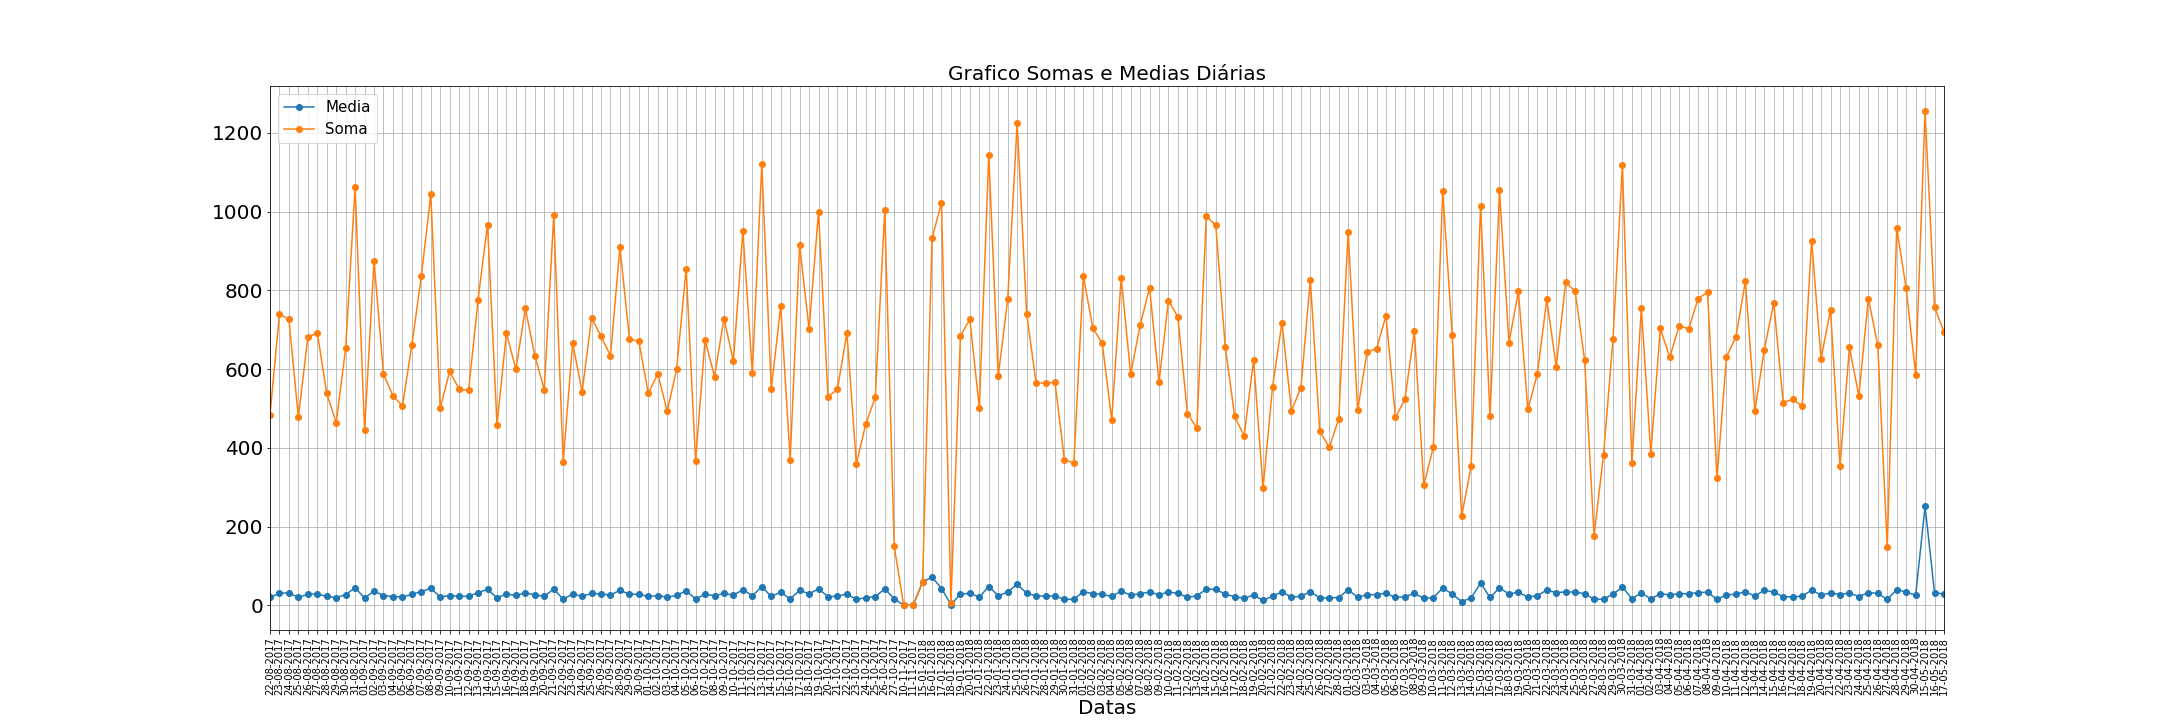
\includegraphics[width=\textwidth,height=\textheight , keepaspectratio]{figuras/GraficoSomaseMediasDiarias(este)}
		\label{graf_total_diaria}
	%\fonte{\cite{fayyad1996data}}
\end{figure}

\begin{figure}[ht]
	\caption{\textbf{Gráfico detalhado da Total Diário}}
	\centering
		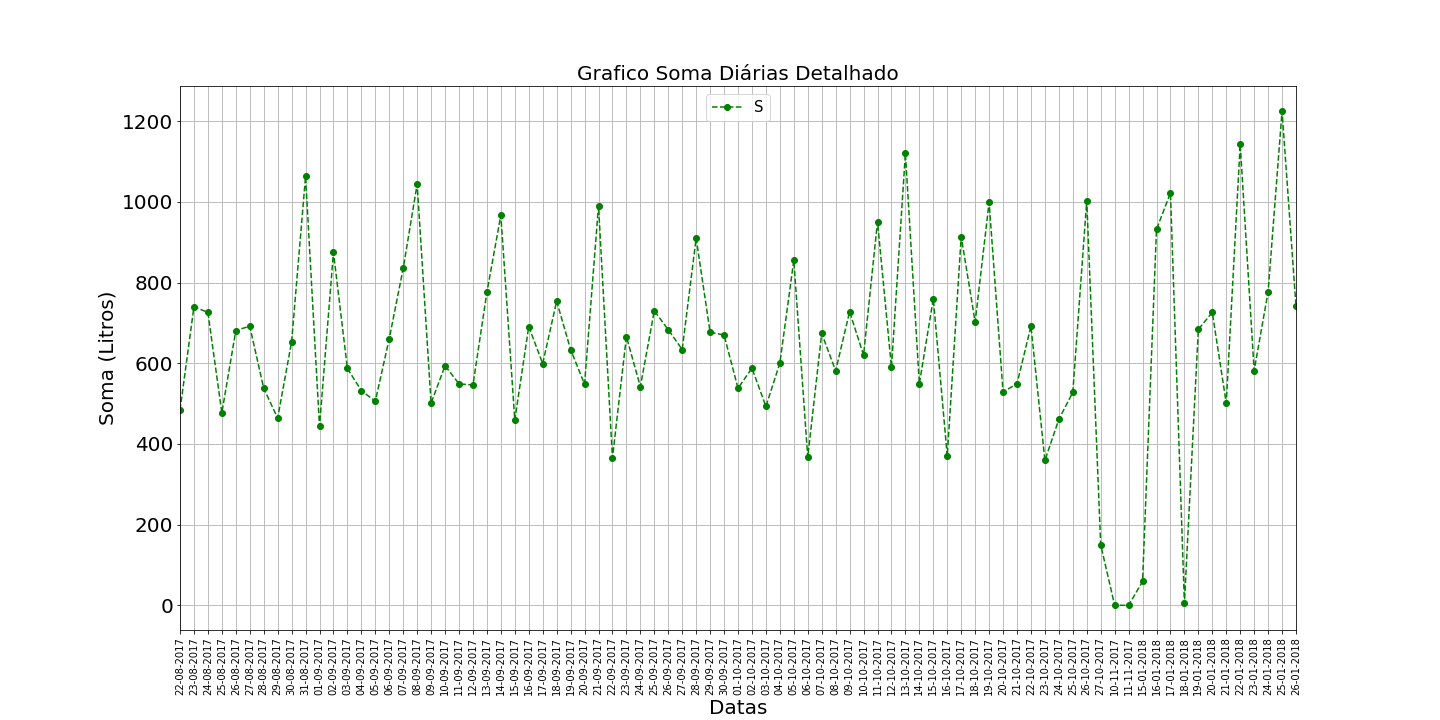
\includegraphics[width=\textwidth,height=\textheight , keepaspectratio]{figuras/GraficoSomaDiarias(estecomzoom)}
		\label{graf_total_diaria_detal}
	%\fonte{\cite{fayyad1996data}}
\end{figure}

\par Utilizando a mesma função detalhada na figura \ref{codigo_medias_diarias}, mas apenas substituindo a função \emph{“mean ()”} pela função \emph{“sum ()”}, foi possível realizar o cálculo do total diário de todo o arquivo. E com a plotagem dos dados obtidos na figura \ref{graf_total_diaria} e na figura \ref{graf_total_diaria_detal}, sendo esta uma plotagem dos dados mais detalhados para verificação, e se observa que na maioria dos dias o consumo ultrapassa 800 litros. Como já mencionado, foi constatado que nesse período dos dados não houve vazamentos, mas não pode se afirmar com certeza se houve excesso no consumo, pois teria que se fazer um estudo aprofundado obtendo o número de consumidores desse local onde foram obtidos os dados.  

\begin{figure}[ht]
	\caption{\textbf{Gráfico do Total Diário entre dois meses com Distância Euclidiana}}
	\centering
		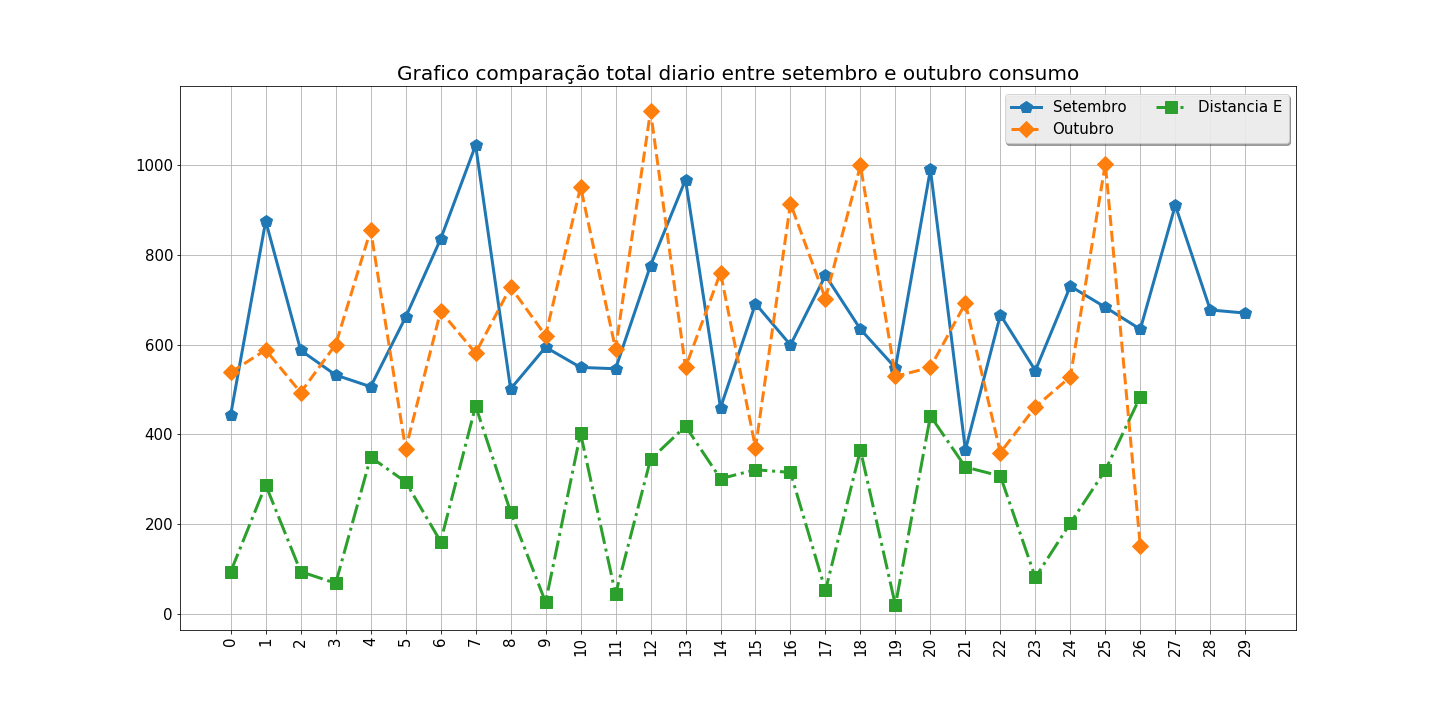
\includegraphics[width=\textwidth,height=\textheight , keepaspectratio]{figuras/comparacaototaldiarioentredoismesesconsumocomdistanciae}
		\label{graf_total_diaria_meses_d}
	%\fonte{\cite{fayyad1996data}}
\end{figure}

\par Com a figura \ref{graf_total_diaria_meses_d} pode se verificar a comparação do total diário entre os meses de setembro e outubro e junto realizado o cálculo com a Distância Euclidiana ponto a ponto e em alguns pontos os resultados se aproxima de zero e observando a semelhança entre os dados.

\begin{figure}[ht]
	\caption{\textbf{Gráfico Simulação de vazamento}}
	\centering
		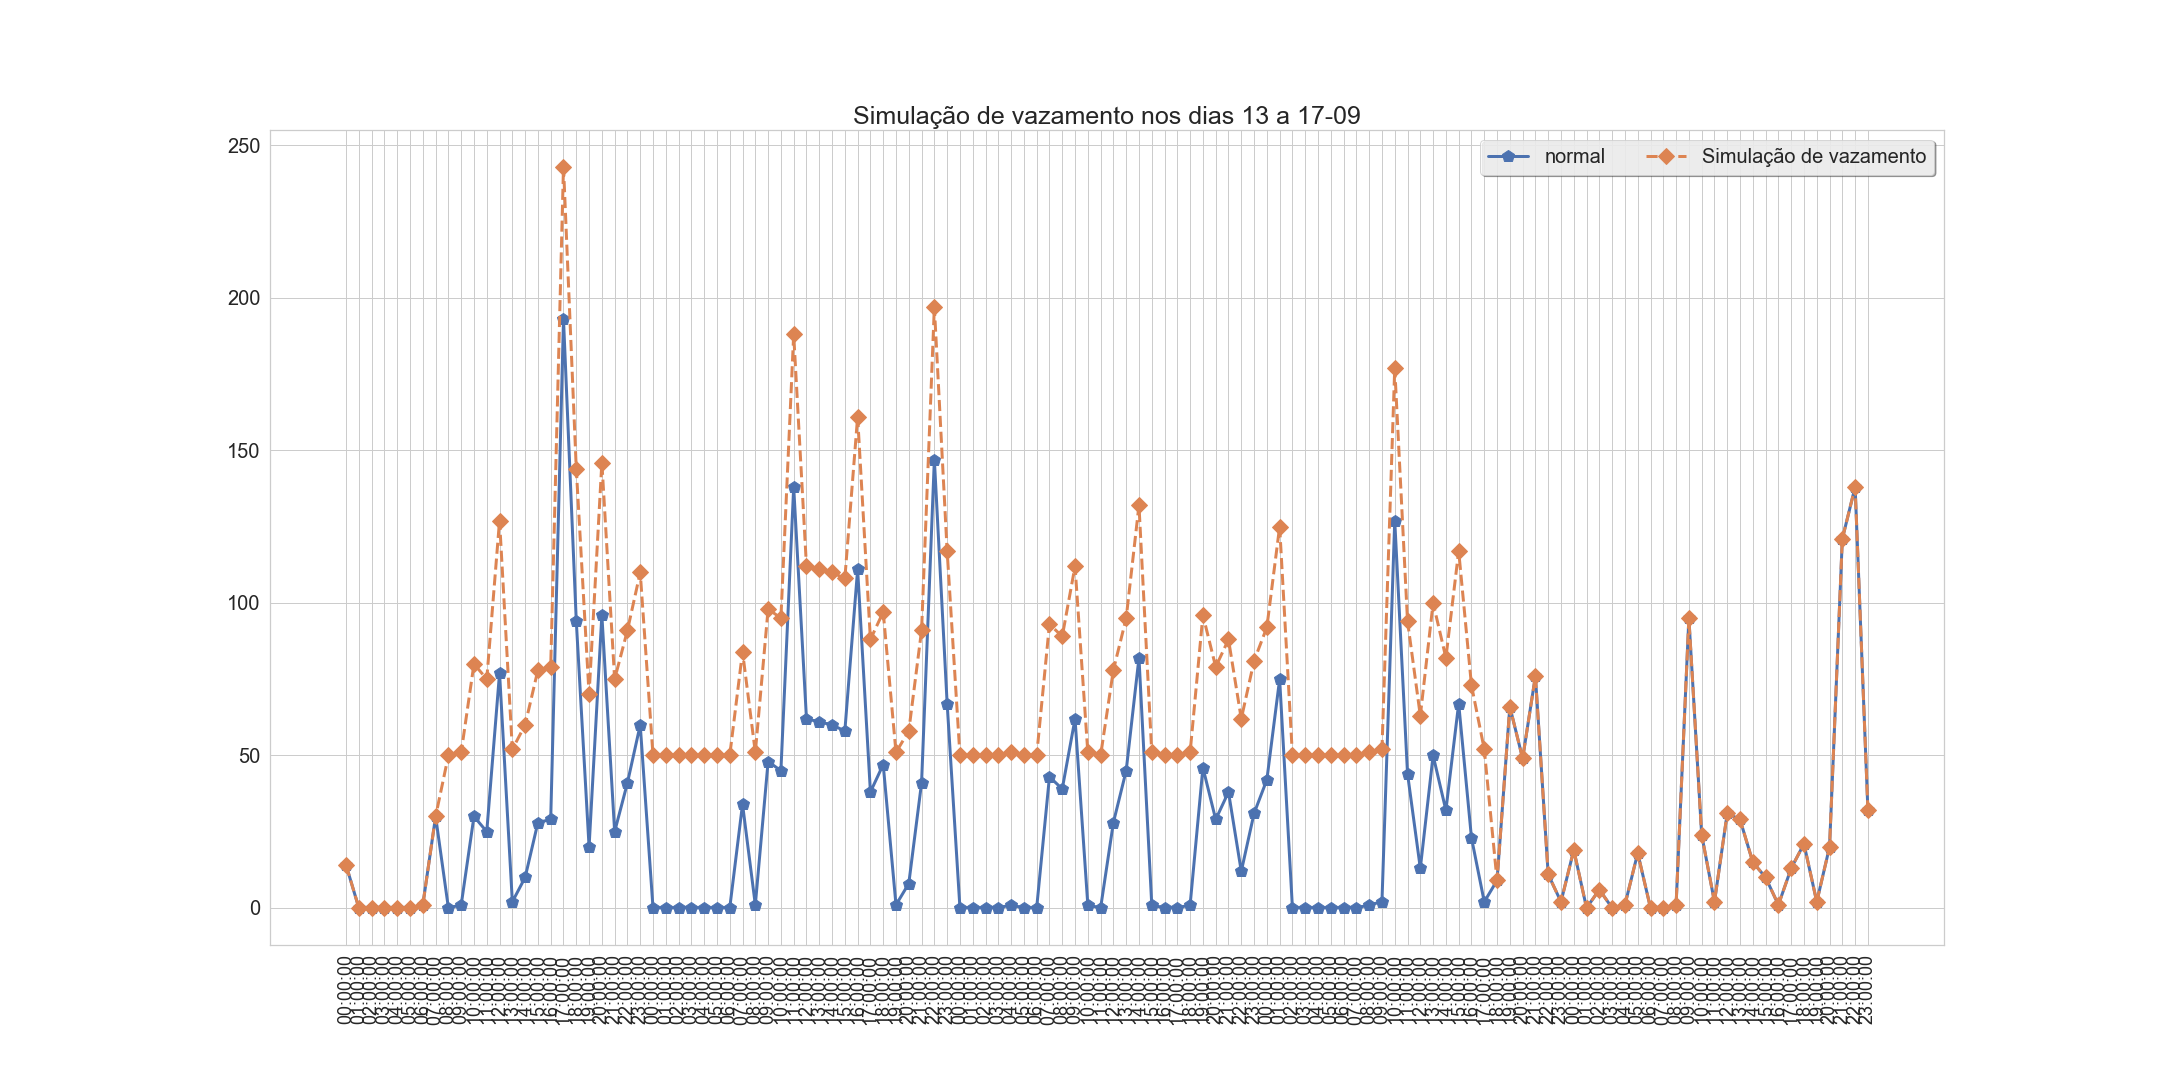
\includegraphics[width=\textwidth,height=\textheight , keepaspectratio]{figuras/Simulacaodevazamentonosdias13a17-09}
		\label{graf_simula_vaz}
	%\fonte{\cite{fayyad1996data}}
\end{figure}

\par O gráfico da figura \ref{graf_simula_vaz} é uma simulação de vazamento. Onde os dados desse mesmo mês foi acrescentada uma constante no valor 50 litros hora e aplicado o resultado desses dados no algoritmo de plotagem da figura \ref{codigo_plotagem}.  Verifica-se que continua tendo o consumo normal, mas há um aumento expressivo  por causa do vazamento. E no final após o vazamento ter sanado retorna-se ao consumo normal. E observando consumo do local onde foram extraídos os dados, o algoritmo apontou neste caso que houve um vazamento, e também apontou-nos outros casos momentos que não houve consumo e momentos onde o consumo se teve picos podendo ser ou não excesso no consumo.

\begin{figure}[ht]
	\caption{\textbf{Simulação de vazamento}}
	\centering
		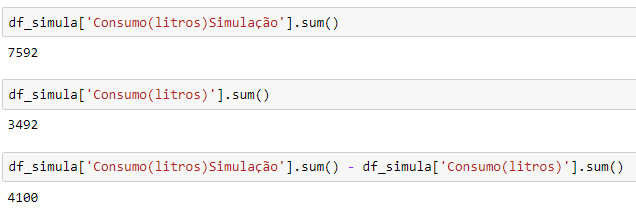
\includegraphics[width=\textwidth,height=\textheight , keepaspectratio]{figuras/somaediferencadasimulacao}
		\label{simula_vaz}
	%\fonte{\cite{fayyad1996data}}
\end{figure}

\par E com a figura \ref{simula_vaz} nota-se que o total de litros acumulados na simulação foi de 7592 litros, em comparação com o total consumido normalmente de 3492 litros, e a diferença entre a simulação e consumo normal é de 4100 litros.

\begin{figure}[ht]
	\caption{\textbf{Gráfico com a simulação de vazamento com distância euclidiana}}
	\centering
		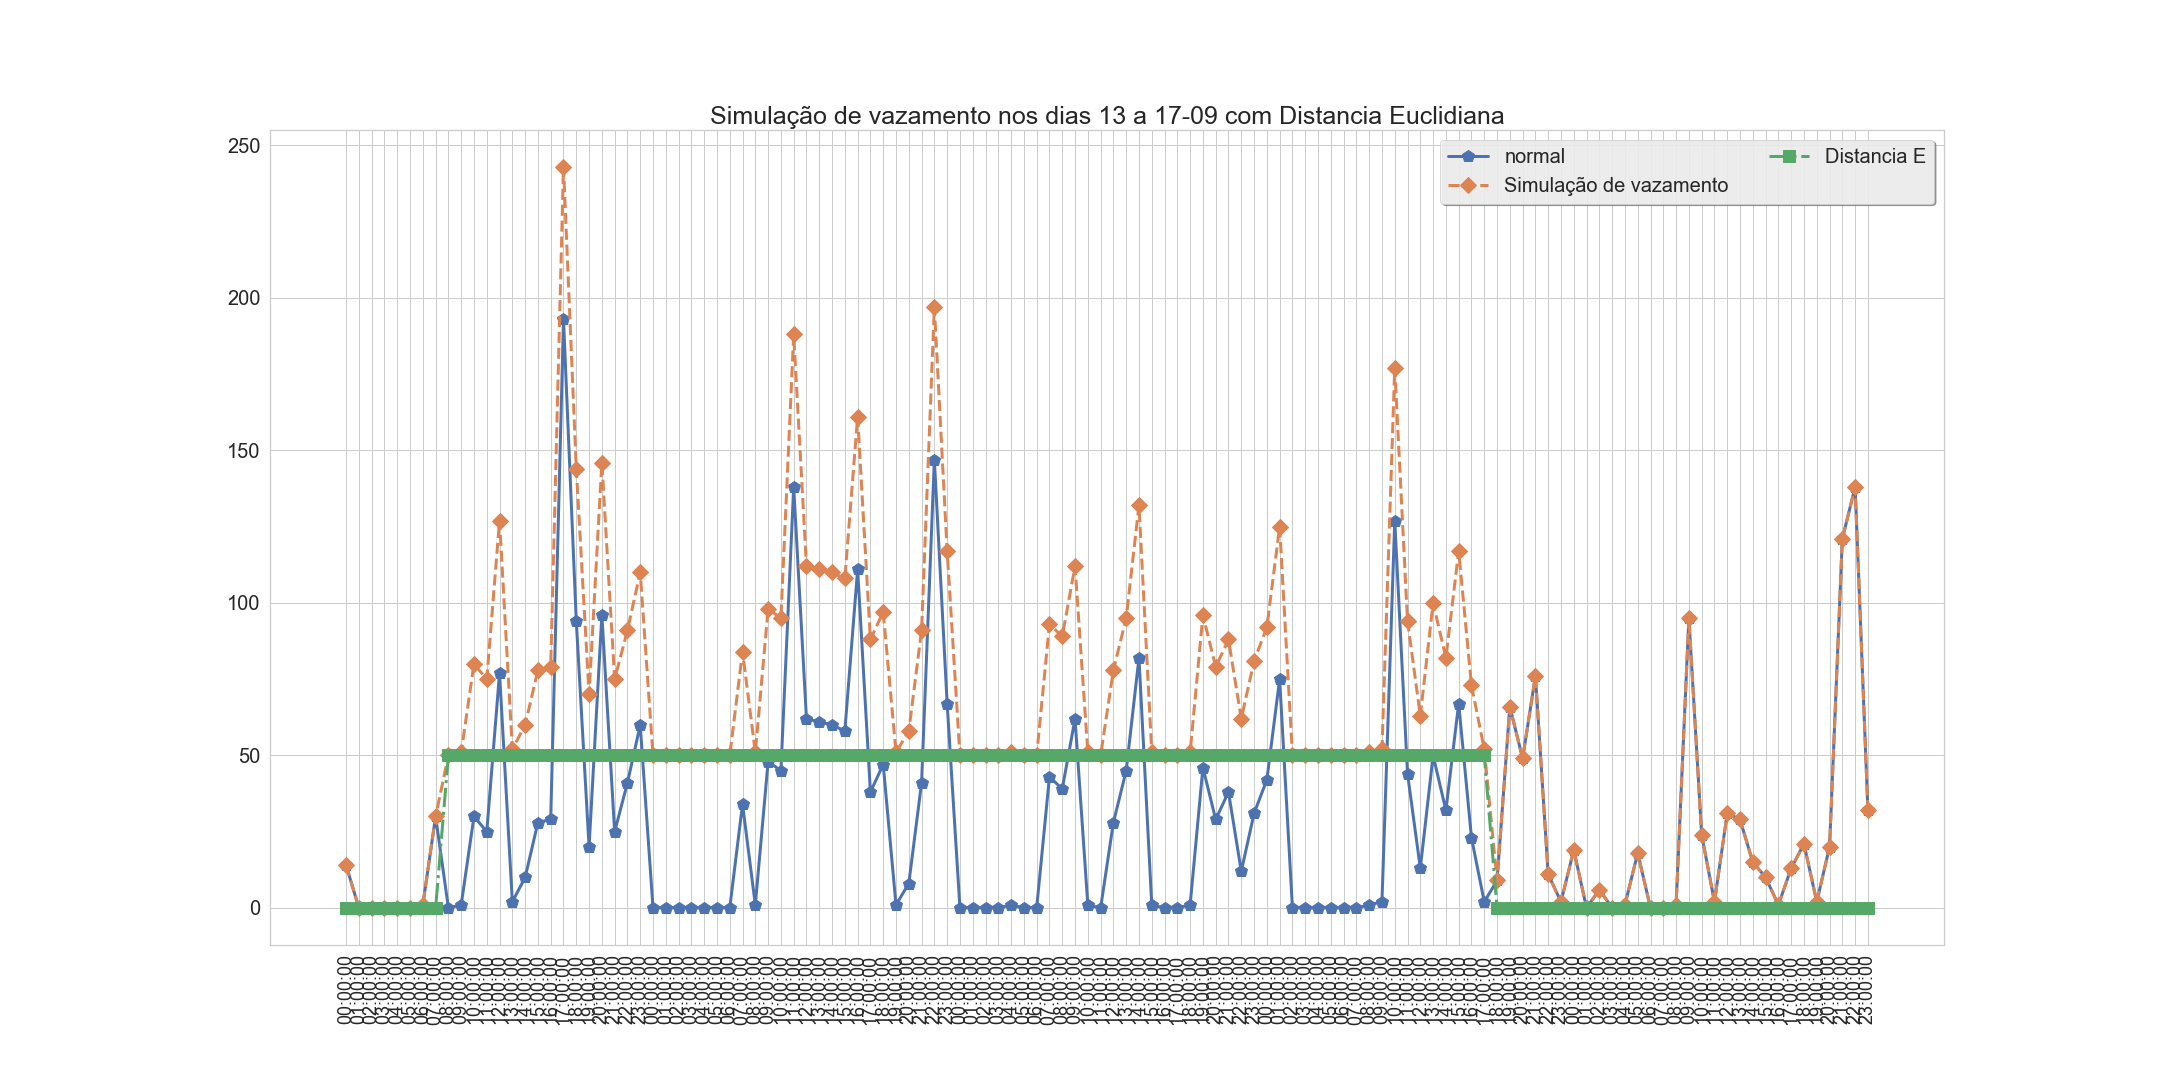
\includegraphics[width=\textwidth,height=\textheight , keepaspectratio]{figuras/Simulacaodevazamentonosdias13a17-09comDistanciaEuclidiana}
		\label{graf_simula_vaz_d}
	%\fonte{\cite{fayyad1996data}}
\end{figure}

\par A figura \ref{graf_simula_vaz_d} apresenta a mesma figura \ref{graf_simula_vaz} com uma diferença o cálculo da Distância Euclidiana ponto a ponto, pode se notar que com o cálculo houve uma ascensão dos pontos no gráfico indicando um aumento no consumo. E voltando ao estado normal assim que o problema foi sanado.

\begin{figure}[ht]
	\caption{\textbf{Gráfico da média hora a hora do arquivo todo}}
	\centering
		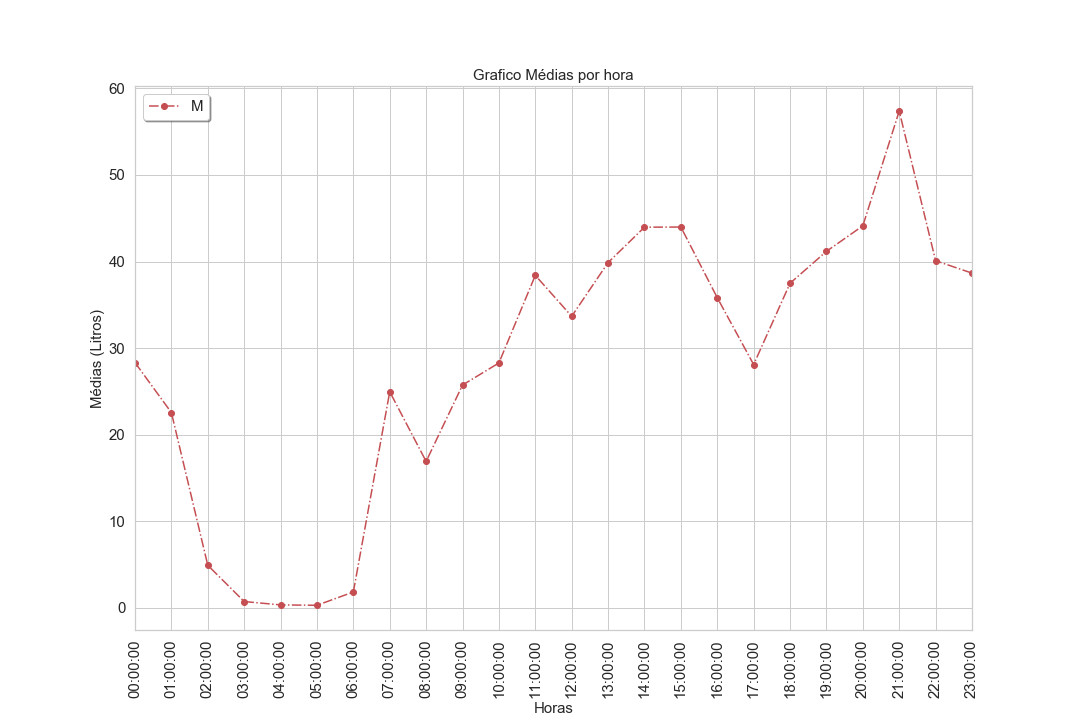
\includegraphics[width=\textwidth,height=\textheight , keepaspectratio]{figuras/GraficoMediasPorHora(este)}
		\label{graf_media_h_h}
	%\fonte{\cite{fayyad1996data}}
\end{figure}

\par Com base na função de cálculo de média, da figura \ref{codigo_medias_diarias}, foi realizada uma plotagem dos dados em gráficos com a média hora a hora total do arquivo. Como pode ser observado na figura \ref{graf_media_h_h}, com isso pode se ter uma base para estipular excesso no consumo de água. 

\begin{figure}[ht]
	\caption{\textbf{Gráfico da média hora a hora entre Fevereiro e Março e a média do arquivo todo}}
	\centering
		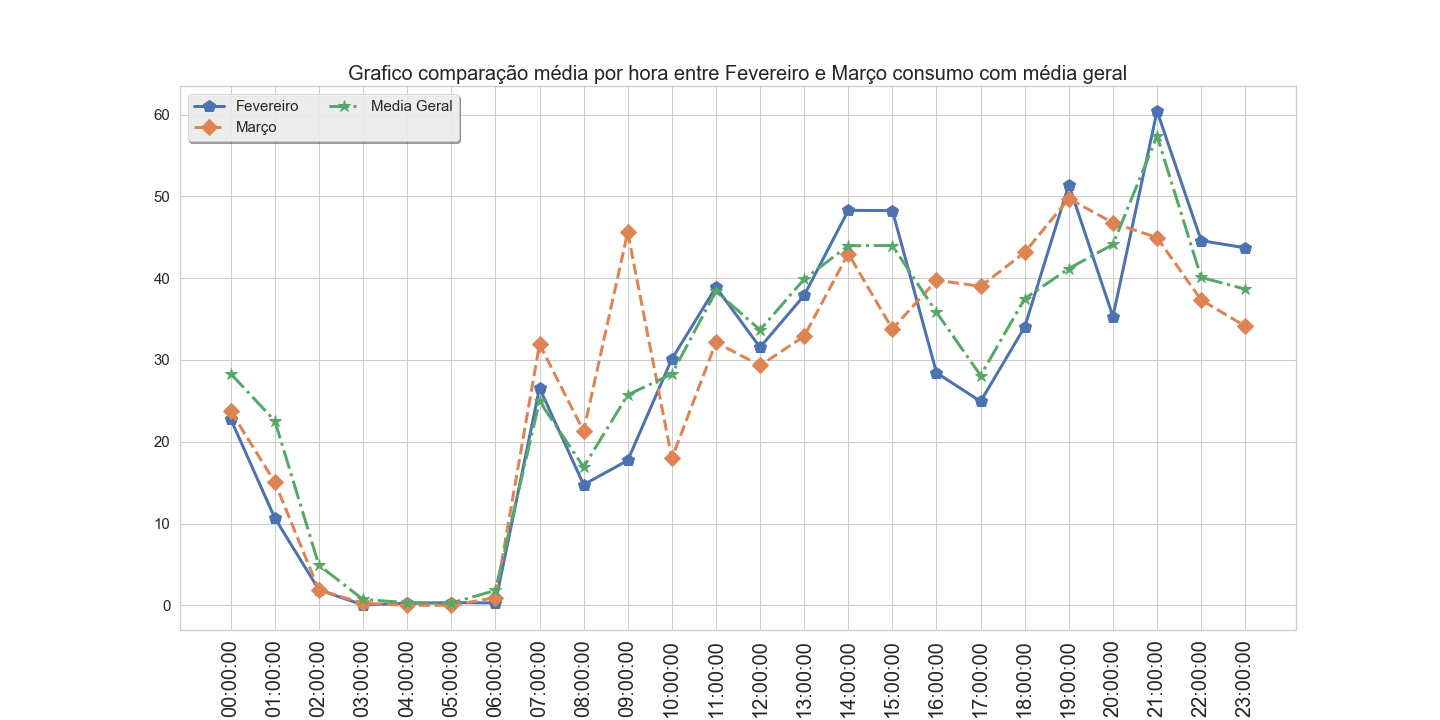
\includegraphics[width=\textwidth,height=\textheight , keepaspectratio]{figuras/comparacaomediahorarientredoismesesconsumo}
		\label{graf_media_h_h_2meses}
	%\fonte{\cite{fayyad1996data}}
\end{figure}

\par Com o gráfico da figura \ref{graf_media_h_h_2meses}, é a plotagem dos dados da comparação entre os meses de Fevereiro e Março de 2018 mais a média de todo o arquivo de dados, pode se observar há períodos semelhantes no consumo de água.

\begin{figure}[h]
	\caption{\textbf{Gráfico da média hora a hora entre Fevereiro, Março e Abril e a média do arquivo todo}}
	\centering
		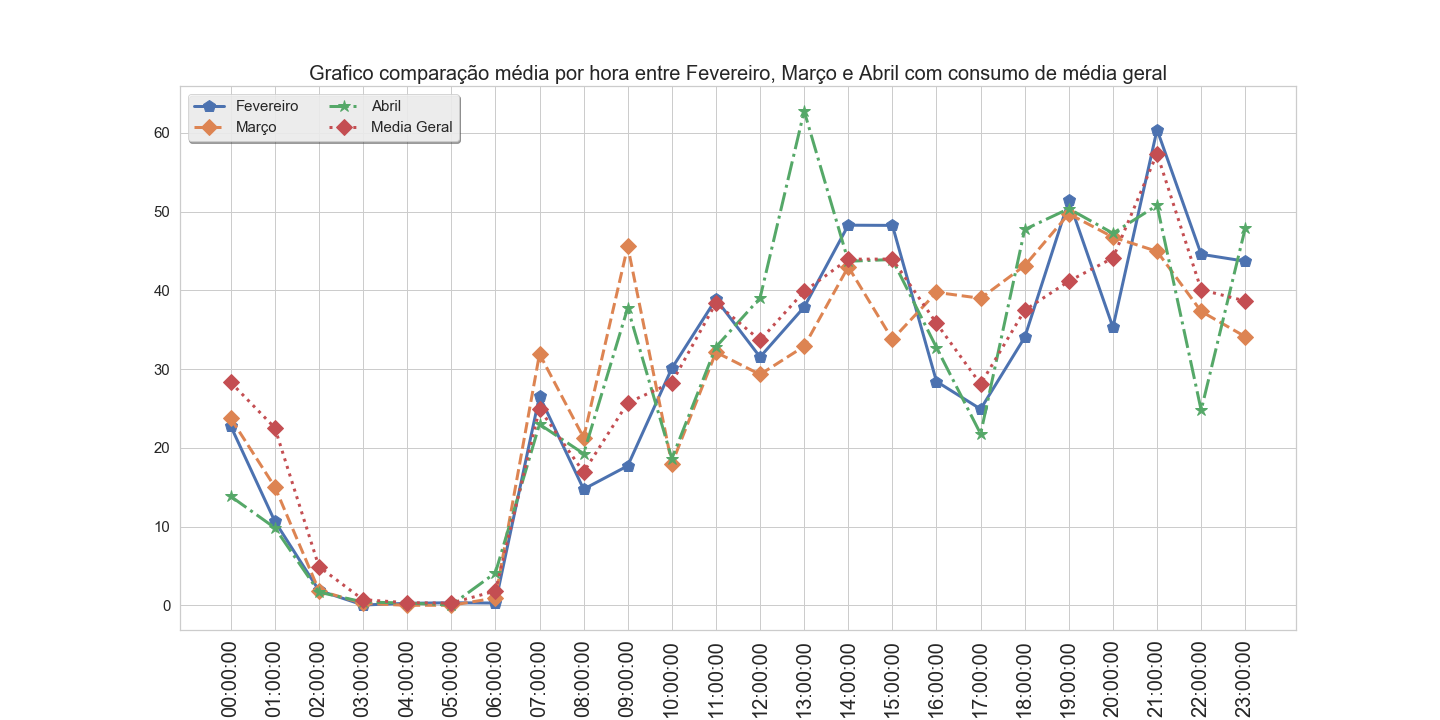
\includegraphics[width=\textwidth,height=\textheight , keepaspectratio]{figuras/comparacaomediahorarientretresmesesconsumo}
		\label{graf_media_h_h_3meses}
	%\fonte{\cite{fayyad1996data}}
\end{figure}

\par Com o gráfico da figura \ref{graf_media_h_h_3meses}, é a plotagem dos dados da comparação entre os meses de Fevereiro, Março e Abril de 2018 mais a média de todo o arquivo de dados, pode se observar há períodos semelhantes no consumo de água. 

% ---

% ---
% Incluindo Capitulo 5 - Conclusao
    \newpage
\chapter{Conclusão}
\par Este trabalho foi desenvolvido para atender as necessidades da empresa TecSUS, utilizando os dados da empresa para realizar um estudo no consumo de água para investigação de detecção possível excesso e vazamento em residências e empresas, visando economia no consumo de água. Utilizando  algumas técnicas de \emph{Data Mining} para plotagem de gráficos, e aplicando a fórmula da Distância Euclidiana. 

\par Tendo em vista  os experimentos aplicados nos dados e os resultados dos gráficos de comparação nos dias da semana, afirma-se que  em alguns períodos não há consumo de água, sendo assim nesses períodos  não houve vazamentos.
 
\par Reforçando que na média geral de todo o arquivo o consumo ficou menor que 30 litros, e nas médias diárias pode se observar que o consumo fica abaixo de 50 litros. E que no acumulado diário o consumo ultrapassa os 800 litros.

\par E aplicando o algoritmo de plotagem nos dados de simulação de vazamento figura \ref{graf_simula_vaz}, obtém um gráfico de simulação de um vazamento, notando que houve um aumento expressivo no consumo de água e retornando ao estado de normalidade quando o problema estiver sanado. E observando  na figura \ref{simula_vaz} onde é feita a soma do total dos litros consumidos e dos litros da simulação do vazamento, e veja  a diferença entre os dois resultados, é verificado que tem um desperdício e assim ocasionando um aumento relativo na conta. E na figura \ref{graf_simula_vaz_d} onde é aplicada a Distância Euclidiana observa se que houve um deslocamento na linha apontando o  aumento no consumo de água ocasionado pelo vazamento, e retornando a normalidade depois que o problema foi sanado.

\par E ao utilizar a fórmula matemática da Distância Euclidiana, que é muito utilizada para análise de séries temporal, o resultado tende ser o mais próximo de zero. E que quanto maior o valor observado menos semelhante será a séries temporal. E que foi possível observar os resultados no decorrer desses dados, que há períodos semelhantes no consumo.

\par E  para realizar previsões para advertir o consumidor caso tivesse um excesso no consumo é necessário uma análise mais profunda, com mais período de dados.


\section{Trabalhos Futuros}
\par Este trabalho expande a possibilidade de melhorias e oportunidade para novas implementações das técnicas. Sendo eles:
\begin{enumerate}
\item  Estudar mais a fundo os dados de  consumo para poder obter mais detalhes para que se possa obter talvez uma previsão nos dados.
\item  Aplicar as técnicas de data mining para outro serviço da empresa TecSUS como sendo o TecLux;
\item  Aplicar as técnicas de data mining para outro serviço da empresa TecSUS como sendo o TecGas;  
\end{enumerate}
   
   
    
% ---

% ---
% Referências bibliográficas
\bibliography{referencias.bib}
% ---
\end{document}
